% !TeX program = pdfLaTeX
\documentclass[12pt]{article}
\usepackage{amsmath}
\usepackage{graphicx,psfrag,epsf}
\usepackage{enumerate}
\usepackage{natbib}
\usepackage{textcomp}
\usepackage[hyphens]{url} % not crucial - just used below for the URL
\usepackage{hyperref}
\providecommand{\tightlist}{%
  \setlength{\itemsep}{0pt}\setlength{\parskip}{0pt}}

%\pdfminorversion=4
% NOTE: To produce blinded version, replace "0" with "1" below.
\newcommand{\blind}{0}

% DON'T change margins - should be 1 inch all around.
\addtolength{\oddsidemargin}{-.5in}%
\addtolength{\evensidemargin}{-.5in}%
\addtolength{\textwidth}{1in}%
\addtolength{\textheight}{1.3in}%
\addtolength{\topmargin}{-.8in}%

%% load any required packages here




\usepackage{float}
\usepackage{bbold}
\usepackage{subfig}
\usepackage{graphicx}
\usepackage[utf8]{inputenc}
\usepackage[T1]{fontenc}
\usepackage{booktabs}
\usepackage{algorithm2e}
\usepackage{caption}
\usepackage{tabularx}
\usepackage{verbatim}
\usepackage{xcolor}
\newcommand{\var}{\mathrm{Var}}

\begin{document}


\def\spacingset#1{\renewcommand{\baselinestretch}%
{#1}\small\normalsize} \spacingset{1}


%%%%%%%%%%%%%%%%%%%%%%%%%%%%%%%%%%%%%%%%%%%%%%%%%%%%%%%%%%%%%%%%%%%%%%%%%%%%%%

\if0\blind
{
  \title{\bf A generalization of partial least squares regression and correspondence
analysis for categorical and mixed data: An application with the ADNI
data}

  \author{
        Derek Beaton \\
    Rotman Research Institute, Baycrest Health Sciences\\
     and \\     ADNI \thanks{Data used in preparation of this article were obtained from the
Alzheimer's Disease Neuroimaging Initiative (ADNI) database
(\url{http://adni.loni.usc.edu/}). As such, the investigators within the
ADNI contributed to the design and implementation of ADNI and/or
provided data but did not participate in analysis or writing of this
report. A complete listing of ADNI investigators can be found at
http://adni.loni.ucla.edu/wpcontent/uploads/how\_to\_apply/ADNI\_Acknowledgement\_List.pdf} \\
    ADNI\\
     and \\     Gilbert Saporta \\
    Conservatoire National des Arts et Metiers\\
     and \\     Hervé Abdi \\
    Behavioral and Brain Sciences, The University of Texas at Dallas\\
      }
  \maketitle
} \fi

\if1\blind
{
  \bigskip
  \bigskip
  \bigskip
  \begin{center}
    {\LARGE\bf A generalization of partial least squares regression and correspondence
analysis for categorical and mixed data: An application with the ADNI
data}
  \end{center}
  \medskip
} \fi

\bigskip
\begin{abstract}
Current large scale studies of brain and behavior typically involve
multiple populations, diverse types of data (e.g., genetics, brain
structure, behavior, demographics, or ``mutli-omics,'' and
``deep-phenotyping'') measured on various scales of measurement. To
analyze these heterogeneous data sets we need simple but flexible
methods able to integrate the inherent properties of these complex data
sets. Here we introduce partial least squares-correspondence
analysis-regression (PLS-CA-R) a method designed to address these
constraints. PLS-CA-R generalizes PLS regression to most data types
(e.g., continuous, ordinal, categorical, non-negative values). We also
show that PLS-CA-R generalizes many ``two-table'' multivariate
techniques and their respective algorithms, such as various PLS
approaches, canonical correlation analysis, and redundancy analysis
(a.k.a. reduced rank regression).
\end{abstract}

\noindent%
{\it Keywords:} generalized singular value decomposition, latent models, genetics, neuroimaging, canonical correlation analysis
\vfill

\newpage
\spacingset{1.45} % DON'T change the spacing!

\hypertarget{introduction}{%
\section{Introduction}\label{introduction}}

\label{section:Intro}

Today's large scale and multi-site studies, such as the UK BioBank
(\url{https://www.ukbiobank.ac.uk/}) and the Rotterdam study
(\url{http://www.erasmus-epidemiology.nl/}), collect population level
data across numerous types and modalities, (e.g., genetics,
neurological, behavioral, clinical, and laboratory measures). Other
types of large scale studies---typically those that emphasize diseases
and disorders---involve a relatively small of participants but collect a
very large number of measures on diverse modalities. Some such studies
include the Ontario Neurodegenerative Disease Research Initiative
(ONDRI) \citep{farhan_ontario_2016} which includes genetics, multiple
types of magnetic resonance brain imaging
\citep{duchesne_canadian_2019}, a wide array of behavioral, cognitive,
clinical, and laboratory batteries, as well as many modalities
``between'' these types, such as ocular imaging, gait, and balance
\citep{montero-odasso_motor_2017-1}, eye tracking, and neuro-pathology.
Though large samples (e.g., UK BioBank) and depth of data (e.g., ONDRI)
are necessary to understand typical and disordered samples and
populations, few statistical or machine learning approaches exist 1)
that can accommodate such large (whether ``big'' or ``wide''), complex,
and heterogeneous data sets and 2) that also respect the inherent
properties of such data.

In many cases, the analysis of a mixture of data types loses information
in part because the data need to be transformed to fit the analytical
methods; but this analysis also loses inferential power because the
standard assumptions may be inappropriate or incorrect. For example, to
analyze categorical and continuous data together, a typical---but
inappropriate---strategy is to recode the continuous data into
categories such as dichotomization, trichotomization, or other (often
arbitrary) binning strategies. Furthermore, ordinal and Likert scale
data---such as responses on many cognitive, behavioral, clinical, and
survey instruments---are often incorrectly treated as metric or
continuous values \citep{burkner_ordinal_nodate}. When it comes to
genetic data, such as single nucleotide polymorphims (SNPs), the data
are almost always recoded by counting the number of the minor homozygote
to give: 0 for the major homozygote (two copies of the most frequent of
the two alleles), 1 for the heterozygote, and 2 for the minor
homozygote. This \{0, 1, 2\} recoding of genotypes (1) assumes additive
linear effects based on the minor homozygote and (2) is often treated as
metric/continuous values (as opposed to categorical or ordinal), even
when known effects of risk are neither linear nor additive, such as
haplotypic effects \citep{vormfelde_value_2007} nor exclusively based on
the minor homozygotes, such as ApoE in Alzheimer's Disease
\citep{genin_apoe_2011}. Interestingly other, less restrictive, models
(e.g., dominant, recessive, genotypic) perform better
\citep{lettre2007genetic} than the additive model, but these are rarely
used.

Here we introduce partial least squares-correspondence
analysis-regression (PLS-CA-R): a latent variable regression modeling
approach suited for the analysis of complex data sets. We first show
that PLS-CA-R generalizes PLS regression
\citep{wold_soft_1975, wold_collinearity_1984, tenenhaus_regression_1998, abdi_partial_2010-1},
CA
\citep{greenacre_theory_1984, greenacre_correspondence_2010-1, lebart_multivariate_1984},
and PLS-CA \citep{beaton_partial_2016}---which is the ``correlation''
companion and basis of PLS-CA-R. We then show that PLS-CA-R is a
data-type general PLS regression method based on the generalized
singular value decomposition (GSVD) that combines the features of CA (to
accommodate multiple data types) with the features of PLS-R (as a
regression method generalizing ordinary least squares regression when
its assumptions are not met).

We illustrate the multiple uses of PLS-CA-R, with data from the
Alzheimer's Disease Neuroimaging Initiative (ADNI). These data include:
diagnosis data (mutually exclusive categories), SNPs (genotypes are
categorical), multiple behavioral or clinical instruments (that could be
ordinal, categorical, or continuous), and several neuroimaging measures
and indices (generally either continuous or non-negative). PLS-CA-R can
1) accommodate these different data types in a predictive or fitting
framework, 2) regress (i.e., residualize) confounds out of mixed and
collinear data, and 3) reveal latent variables within a well-established
framework.

Finally, we show that PLS-CA-R can be generalized 1) to handle multiple
data types, 2) various optimization schemes(e.g., covariance as in PLS
or correlation as in canonical correlation), 3) various transformations
for alternate metrics, and 4) ridge-like regularization and 5) multiple
PLS algorithms.

This paper is organized as follows. In Section \ref{section:PLSCAR} we
introduce PLS-CA-R. Next, in Section \ref{section:appex}, we illustrate
PLS-CA-R on the TADPOLE challenge
(\url{https://tadpole.grand-challenge.org/}) and additional genetics
data from ADNI across three examples: 1) a simple discriminant example
with categorical data, 2) a mixed data example that requires
residualization (i.e., adjusting for confounds), and 3) a larger example
of multiple genetic markers and whole brain tracer uptake (non-negative
values). Finally in Section \ref{section:Disc} we discuss PLS-CA-R, and
show how PLS-CA-R generalizes the PLS framework to multiple optimization
problems, algorithms, metrics, and ridge-like regularization.

\hypertarget{partial-least-squares-correspondence-analysis-regression}{%
\section{Partial least squares-correspondence
analysis-regression}\label{partial-least-squares-correspondence-analysis-regression}}

\label{section:PLSCAR}

Here we present the generalization of partial least square-regression
(PLS-R) to multiple correspondence analysis (MCA) and correspondence
analysis (CA)-like problems that generally apply to categorical
(nominal) data. Via CA, we can also generalize to other data types
including mixed types (e.g., categorical, ordinal, continuous,
contingency). We use a mixture of nomenclature associated with
\(\chi^2\)-analyses, CA, and PLS-R.

\hypertarget{pls-algorithms}{%
\subsection{PLS algorithms}\label{pls-algorithms}}

There exist three commonly used PLS algorithms: (1) PLS ``correlation''
decomposition
\citetext{\citealp[partial\_2011]{krishnan}; \citealp{bookstein1994partial}; \citealp[spatial\_1996]{mcintosh}}---also
known as PLSSVD \citep[regression\_1998]{tenenhaus} or Tucker's
Interbattery Factor Analysis \citep[inter-battery\_1958]{tucker}, (2)
PLS ``canonical'' decompostion \citep[regression\_1998]{tenenhaus}, and
(3) PLS ``regression''
\citetext{\citealp[soft\_1975]{wold}; \citealp[collinearity\_1984]{wold}; \citealp[pls-regression\_2001]{wold}}.
PLS correlation decomposition is a symmetric method where neither data
table plays a privileged (or predictive) role, and is performed with a
single pass of the singular value decomposition (SVD). PLS canonical
decomposition is also symmetric, but makes use of the SVD iteratively
and deflates both data tables in each iteration. PLS regression
decomposition is an asymmetric method where one data table is privileged
(``predictors'') and also makes use of the SVD iteratively with
deflation of both data tables.

\hypertarget{notation}{%
\subsection{Notation}\label{notation}}

Bold uppercase letters denote matrices (e.g., \(\mathbf{X}\)), bold
lowercase letters denote vectors (e.g., \(\bf{x}\)), and italic
lowercase letters denote specific elements (e.g., \(x\)). Upper case
italic letters (e.g., \(I\)) denote cardinality, size, or length where a
lower case italic (e.g., \(i\)) denotes a specific value of an index. A
generic element of matrix \(\mathbf{X}\) would be denoted \(x_{i,j}\).
Common letters of varying type faces, for example \({\bf X}\),
\(\bf{x}\), \(x_{i,j}\), come from the same data structure. A
preprocessed or transformed version of a matrix \({\mathbf X}\) is
denoted \({\mathbf Z}_{\mathbf X}\). Vectors are assumed to be column
vectors unless otherwise specified. Two matrices side-by-side denotes
standard matrix multiplication (e.g., \(\bf{X}\bf{Y}\)). The operator
\(\odot\) denotes element-wise (Hadamard) multiplication and \(\oslash\)
denotes element-wise (Hadamard) division. The matrix \({\bf I}\) denotes
the identity matrix, \(\mathbf{1}\) and \(\mathbf{0}\) denote
respectivvely a vector or marix of 1's or 0. Superscript \(^{T}\)
denotes the transpose operation, superscript \(^{-1}\) denotes standard
matrix inversion, and superscript \(^{+}\) denotes the Moore-Penrose
pseudo-inverse. The diagonal operator, denoted \(\mathrm{diag\{\}}\),
transforms a vector into a diagonal matrix, or extracts the diagonal of
a matrix to produce a vector.

\hypertarget{the-svd-gsvd-ca-and-gplssvd}{%
\subsection{The SVD, GSVD, CA, and
GPLSSVD}\label{the-svd-gsvd-ca-and-gplssvd}}

\label{section:GSVDCA}

Let \({\mathbf X}\) be a data matrix with \(I\) rows and \(J\) columns,
\({\mathbf X}\) is preprocessed in some way to give
\({\mathbf Z}_{\mathbf X}\). The singular value decomposition (SVD)
decomposes \({\mathbf Z}_{\mathbf X}\) as \begin{equation}\label{eq:svd}
{\mathbf Z}_{\mathbf X} = 
{\mathbf U} {\boldsymbol \Delta} {\mathbf V}^{T}
\textrm{ with } {\mathbf U}^{T}{\mathbf U} 
= {\mathbf I} = {\mathbf V}^{T}{\mathbf V},
\end{equation} where \({\mathbf Z}_{\mathbf X}\) is of rank \(A\) (with
\(A \leq \min(I,J)\)) and \({\boldsymbol \Delta}\) is the \(A \times A\)
diagonal matrix of the singular values, and
\({\boldsymbol \Lambda} = {\boldsymbol \Delta}^2\) is the \(A \times A\)
diagonal matrix of the eigenvalues. Matrices \({\mathbf U}\) and
\({\mathbf V}\) store (respectively) the left and right singular vectors
of \({\mathbf Z}\). Component (a.k.a. factor) scores for the \(I\) rows
and \(J\) columns of \({\mathbf Z}_{\mathbf X}\) are computed as
\({\mathbf F}_{I} = {\mathbf U}{\boldsymbol \Delta}\)
\({\mathbf F}_{J} = {\mathbf V}{\boldsymbol \Delta}\).

The \emph{generalized} singular value decomposition (GSVD) generalizes
the SVD by integrating constraints (expressed by positive definite
matrices) also called \emph{metric} (because these matrices define a
metric in a generalized Euclidean space) imposed on the rows and columns
of the matrix to be decomposed. Specifically, if
\({\mathbf M}_{{\mathbf X}}\) (respectively
\({\mathbf W}_{{\mathbf X}}\)) is an \(I\times I\) (respectively
\(J\times J\)) positive definite matrix, the GSVD decomposes
\({\mathbf Z}_{\mathbf X}\) as \begin{equation}\label{eq:gsvd}
{\mathbf Z}_{\mathbf X} = {\mathbf P} 
{\boldsymbol \Delta} {\mathbf Q}^{T} 
\textrm{ with }
{\mathbf P}^{T}{\mathbf M}_{{\mathbf X}}{\mathbf P} = {\mathbf I} = {\mathbf Q}^{T}{\mathbf W}_{{\mathbf X}}{\mathbf Q}
\end{equation} where \({\mathbf Z}_{\mathbf X}\) is of rank \(A\) and
\({\boldsymbol \Delta}\) is the \(A \times A\) diagonal matrix of the
(generalized) singular values and \({\mathbf P}\) and \({\mathbf Q}\)
are the \emph{generalized} singular vectors. We refer to a more
convenient expression of the GSVD with ``triplet notation''
\citep[\citet{holmes_multivariate_2008},\citet{dray2014}]{escoufier2006}
but in the form of
\(\mathrm{GSVD(} {\mathbf M}_{{\mathbf X}}, {\mathbf Z}_{\mathbf X}, {\mathbf W}_{{\mathbf X}} \mathrm{)}\),
which is akin to how the multiplication steps work \citep[see
also][]{beaton2018generalization}. Note that the standard SVD is the
GSVD but with identity matrices as the weights:
\(\mathrm{GSVD(} {\mathbf I}, {\mathbf X}, {\mathbf I} \mathrm{)}\)
\citep[see also][]{takane_relationships_2003}, and thus if
\({\mathbf Z}_{\mathbf X}\) were a column-wise centered and/or
normalized version of \({\mathbf X}\) then
\(\mathrm{GSVD(} {\mathbf I}, {\mathbf Z}_{\mathbf X}, {\mathbf I} \mathrm{)}\)
implements principal components analysis
\citep[PCA,][\citet{abdi2007svd}]{saporta2011}.

Correspondence analysis (CA) is a technique akin to PCA but initially
designed for contingency and nominal data, and operates under the
assumption of indepdence (i.e., akin to \(\chi^2\)). See
\citet{greenacre_theory_1984}, \citet{greenacre_correspondence_2010-1},
and \citet{lebart_multivariate_1984} for detailed explanations of CA,
and then see \citet{escofier-cordier_analyse_1965} and
\citet{benzecri_analyse_1973} for the origins and early developments of
CA. Assume the matrix \({\mathbf X}\) is some \(I \times J\) matrix
comprised of non-negative data (e.g., counts or categorical data
expressed in disjunctive format as, e.g., ``SEX'' in Table
\ref{table:disj}).

CA is performed with the GSVD as follows. First the \emph{observed}
probability matrix is computed as
\({\mathbf O}_{\mathbf X} = {\mathbf X} \times ({\mathbf 1}^{T}{\mathbf X} {\mathbf 1})^{-1}\)
The marginal probabilities from the observed matrix ar then computed as
\begin{equation}
{\mathbf m}_{\mathbf X} = {\mathbf O}_{\mathbf X}{\mathbf 1} 
\text{ and } 
{\mathbf w}_{\mathbf X} = ({\mathbf 1}^{T}{\mathbf O}_{\mathbf X})^{T}.
\end{equation} The \emph{expected} (under the assumption of
independence, i.e., \(\chi^2\)) matrix as
\({\mathbf E}_{\mathbf X} = {\mathbf m}_{\mathbf X}{\mathbf w}_{\mathbf X}^{T}\).
The \emph{deviation} from independence matrix is then defined as
\begin{equation}
{\mathbf Z}_{\mathbf X} 
= {\mathbf O}_{\mathbf X} - {\mathbf E}_{\mathbf X}.
\end{equation} Finally, CA is obtained from
\begin{equation}\label{eq:CAasGSVD}
\mathrm{GSVD(} {\mathbf M}_{\mathbf X}^{-1}, 
{\mathbf Z}_{\mathbf X}, {\mathbf W}_{\mathbf X}^{-1} \mathrm{)}
\textrm{ with }
{\mathbf M}_{\mathbf X} 
=  \mathrm{diag\{} {\mathbf m}_{\mathbf X} 
\mathrm{\}} \text{ and } {\mathbf W}_{\mathbf X} 
= \mathrm{diag\{} {\mathbf w}_{\mathbf X} \mathrm{\}}.
\end{equation}

\hypertarget{from-the-triplet-to-the-sextuplet}{%
\subsection{From the triplet to the
sextuplet}\label{from-the-triplet-to-the-sextuplet}}

We now introduce an extension of the GSVD and its triplet concept for
PLS, called the ``GPLSSVD sextuplet'' to decompose the the relationship
between two matrices each with the same \(I\) observations (along the
rows): \({\mathbf X}\) with \(J\) columns and \({\mathbf Y}\) with \(K\)
columns, where \({\mathbf Z}_{\mathbf X}\) and
\({\mathbf Z}_{\mathbf Y}\) are preprocessed versions of \({\mathbf X}\)
and \({\mathbf Y}\), respectively. The ``GPLSSVD sextuplet'' takes the
form of
\(\mathrm{GPLSSVD(} {\mathbf M}_{\mathbf X}, {\mathbf Z}_{\mathbf X}, {\mathbf W}_{\mathbf X}, {\mathbf M}_{\mathbf Y}, {\mathbf Z}_{\mathbf Y}, {\mathbf W}_{\mathbf Y} \mathrm{)}\).
The
\(\mathrm{GPLSSVD(} {\mathbf M}_{\mathbf X}, {\mathbf Z}_{\mathbf X}, {\mathbf W}_{\mathbf X}, {\mathbf M}_{\mathbf Y}, {\mathbf Z}_{\mathbf Y}, {\mathbf W}_{\mathbf Y} \mathrm{)}\)
decomposes the matrix
\({\mathbf Z}_{\mathbf R} = {\mathbf Z}_{\mathbf X} {\mathbf W}_{\mathbf X}^{\frac{1}{2}} {\mathbf M}_{\mathbf Y}^{\frac{1}{2}} {\mathbf Z}_{\mathbf Y}\)
as

\begin{equation}
{\mathbf Z}_{\mathbf R} = {\mathbf P} {\boldsymbol \Delta} {\mathbf Q}^{T}
\textrm{ with }
{\mathbf P}^{T}{\mathbf W}_{\mathbf X}{\mathbf P} = {\mathbf I} =
{\mathbf Q}^{T}{\mathbf W}_{\mathbf Y}{\mathbf Q}.
\end{equation}

From this decomposition, the GPLSSVD creates latent variables as

\begin{equation}
{\mathbf L}_{\mathbf X} 
= {\mathbf Z}_{\mathbf X}{\mathbf W}_{\mathbf X}{\mathbf P} 
\textrm{ and } 
{\mathbf L}_{\mathbf Y} = 
{\mathbf Z}_{\mathbf Y}{\mathbf W}_{\mathbf Y}{\mathbf Q}
\textrm{ where }
{\mathbf L}_{\mathbf X}^{T} {\mathbf L}_{\mathbf Y} 
= {\boldsymbol \Delta}. 
\end{equation}

When \({\mathbf X}\) and \({\mathbf Y}\) are column-wise centered
normalized and when all constraint matrices are equal to the identity
matrix---i.e.,
\(\mathrm{GPLSSVD(} {\mathbf I}, {\mathbf Z}_{\mathbf X}, {\mathbf I}, {\mathbf I}, {\mathbf Z}_{\mathbf Y}, {\mathbf I} \mathrm{)}\)---the
GPLSSVD implements the ``PLS correlation'' decomposition
\citep{krishnan_partial_2011, bookstein1994partial, mcintosh_spatial_1996},
also known as PLSSVD \citep{tenenhaus_regression_1998}, co-inertia
analyses \citep[\citet{dray2014}]{doledec1994}, and originally as
Tucker's interbattery factor analysis \citep{tucker_inter-battery_1958}.

Finally, we also introduce a small modification of the ``triplet'' and
``sextuplet'' notations as a ``quadruplet'' and a ``septuplet'' that
indicate the desired rank to be returned by the GSVD or GPLSSVD. For
example, if we want only one component from either approach we would
indicate the desired rank to return as
\(\mathrm{GSVD(} {\mathbf M}_{{\mathbf X}}, {\mathbf Z}_{\mathbf X}, {\mathbf W}_{{\mathbf X}}, 1 \mathrm{)}\)
and
\(\mathrm{GPLSSVD(} {\mathbf M}_{\mathbf X}, {\mathbf Z}_{\mathbf X}, {\mathbf W}_{\mathbf X}, {\mathbf M}_{\mathbf Y}, {\mathbf Z}_{\mathbf Y}, {\mathbf W}_{\mathbf Y}, 1 \mathrm{)}\).
Both the GSVD and GPLSSVD in these cases would return only one set of
singular vectors, generalized singular vectors, and component scores,
and one singular value; for GPLSSVD it would return only one pair of
latent variables.

\begin{table}[!h]

\caption{\label{tab:unnamed-chunk-1}\label{table:disj} An example of disjunctive (SEX) and pseudo-disjunctive (AGE, EDU) coding through the fuzzy or Escofier transforms. For disjunctive an pseudo-disunctive data, each variable has a row-wise sum of 1 across its respective columns, and thus the row sums across the table are the number of original variables.}
\centering
\begin{tabular}[t]{llrrrrrrrr}
\toprule
\multicolumn{1}{c}{ } & \multicolumn{3}{c}{Original coding} & \multicolumn{6}{c}{Disjunctive and pseudo-disjunctive coding} \\
\cmidrule(l{2pt}r{2pt}){2-4} \cmidrule(l{2pt}r{2pt}){5-10}
\multicolumn{4}{c}{ } & \multicolumn{2}{c}{SEX} & \multicolumn{2}{c}{AGE} & \multicolumn{2}{c}{EDU} \\
\cmidrule(l{2pt}r{2pt}){5-6} \cmidrule(l{2pt}r{2pt}){7-8} \cmidrule(l{2pt}r{2pt}){9-10}
  & SEX & AGE & EDU & Male & Female & AGE- & AGE+ & EDU- & EDU+\\
\midrule
SUBJ 1 & Male & 64.8 & 16 & 1 & 0 & 1.03 & -0.03 & 0.33 & 0.67\\
SUBJ 2 & Female & 63.6 & 18 & 0 & 1 & 1.11 & -0.11 & 0.17 & 0.83\\
SUBJ 3 & Female & 76.4 & 18 & 0 & 1 & 0.24 & 0.76 & 0.17 & 0.83\\
SUBJ 4 & Male & 66.0 & 18 & 1 & 0 & 0.95 & 0.05 & 0.17 & 0.83\\
SUBJ 5 & Female & 61.9 & 14 & 0 & 1 & 1.23 & -0.23 & 0.50 & 0.50\\
\addlinespace
SUBJ 6 & Female & 66.7 & 14 & 0 & 1 & 0.90 & 0.10 & 0.50 & 0.50\\
\bottomrule
\end{tabular}
\end{table}

\hypertarget{pls-ca-r}{%
\subsection{PLS-CA-R}\label{pls-ca-r}}

\label{section:plscar_form}

For simplicity assume in the following formulation that \({\mathbf X}\)
and \({\mathbf Y}\) are both complete disjunctive tables as seen in
Table \ref{table:disj} (see SEX columns) or Table
\ref{table:snps_models_disj}. This formulation also applies generally to
non-negative data (see later sections). We define observed matrices for
\({\mathbf X}\) and \({\mathbf Y}\) as

\begin{equation}
\begin{aligned}
{\mathbf O}_{\mathbf X} = {\mathbf X} \times ({\mathbf 1}^{T}{\mathbf X} {\mathbf 1})^{-1}, \\
{\mathbf O}_{\mathbf Y} = {\mathbf Y} \times ({\mathbf 1}^{T}{\mathbf Y} {\mathbf 1})^{-1}
\label{eq:observedXY}
\end{aligned}
\end{equation} Next we compute marginal probabilities for the rows and
columns. We compute row probabilities as \begin{equation}
{\mathbf m}_{\mathbf X} = {\mathbf O}_{\mathbf X}{\mathbf 1} \text{ and } {\mathbf m}_{\mathbf Y} = {\mathbf O}_{\mathbf Y}{\mathbf 1},
\label{eq:xy_rowvecs}
\end{equation} which are the row sums of the observed matrices in Eq.
\ref{eq:observedXY}. Then we compute column probabilities as
\begin{equation}
{\mathbf w}_{\mathbf X} = ({\mathbf 1}^{T}{\mathbf O}_{\mathbf X})^{T} \text{ and } {\mathbf w}_{\mathbf Y} = ({\mathbf 1}^{T}{\mathbf O}_{\mathbf Y})^{T},
\label{eq:weightmats_v1}
\end{equation} which are the column sums of the observed matrices in Eq.
\ref{eq:observedXY}. We then define expected matrices as
\begin{equation}
{\mathbf E}_{\mathbf X} = {\mathbf m}_{\mathbf X}{\mathbf w}_{\mathbf X}^{T} \text{ and } {\mathbf E}_{\mathbf Y} = {\mathbf m}_{\mathbf Y}{\mathbf w}_{\mathbf Y}^{T},
\label{eq:models}
\end{equation} and deviation matrices as \begin{equation}
{\mathbf Z}_{\mathbf X} = {\mathbf O}_{\mathbf X} - {\mathbf E}_{\mathbf X} \text{ and } {\mathbf Z}_{\mathbf Y} = {\mathbf O}_{\mathbf Y} - {\mathbf E}_{\mathbf Y},
\label{eq:plscar_Zs}
\end{equation}

For PLS-CA-R we have two matrices, \({\mathbf Z}_{\mathbf X}\) which is
\(I \times J\) and \({\mathbf Z}_{\mathbf Y}\) which is \(I \times K\),
and their respective row and column weights of
\({\mathbf M}_{\mathbf X} = \mathrm{diag\{}{\mathbf m}_{\mathbf X} \mathrm{\}}\),
\({\mathbf M}_{\mathbf Y} = \mathrm{diag\{}{\mathbf m}_{\mathbf Y} \mathrm{\}}\),
\({\mathbf W}_{\mathbf X} = \mathrm{diag\{}{\mathbf w}_{\mathbf X} \mathrm{\}}\),
and
\({\mathbf W}_{\mathbf Y} = \mathrm{diag\{}{\mathbf w}_{\mathbf Y} \mathrm{\}}\).
PLS-CA-R makes use of the rank 1 GPLSSVD
iteratively---\(\mathrm{GPLSSVD(} {\mathbf M}_{\mathbf X}^{-1}, {\mathbf Z}_{\mathbf X}, {\mathbf W}_{\mathbf X}^{-1}, {\mathbf M}_{\mathbf Y}^{-1}, {\mathbf Z}_{\mathbf Y}, {\mathbf W}_{\mathbf Y}^{-1}, 1 \mathrm{)}\)---and
works as follows.

First we have
\(\widetilde{{\mathbf Z}}_{\mathbf X} = {\mathbf M}_{\mathbf X}^{-\frac{1}{2}}{\mathbf Z}_{\mathbf X}{\mathbf W}_{\mathbf X}^{-\frac{1}{2}}\)
and
\(\widetilde{{\mathbf Z}}_{\mathbf Y} = {\mathbf M}_{\mathbf Y}^{-\frac{1}{2}}{\mathbf Z}_{\mathbf Y}{\mathbf W}_{\mathbf Y}^{-\frac{1}{2}}\).
Then we compute the cross-product between
\(\widetilde{\mathbf Z}_{\mathbf X}\) and
\(\widetilde{\mathbf Z}_{\mathbf Y}\) as
\({\mathbf Z}_{\mathbf R} = \widetilde{\mathbf Z}_{\mathbf X}^{T}\widetilde{\mathbf Z}_{\mathbf Y} = ({\mathbf M}_{\mathbf X}^{-\frac{1}{2}}{\mathbf Z}_{\mathbf X}{\mathbf W}_{\mathbf X}^{-\frac{1}{2}})^{T}({\mathbf M}_{\mathbf Y}^{-\frac{1}{2}}{\mathbf Z}_{\mathbf Y}{\mathbf W}_{\mathbf Y}^{-\frac{1}{2}})\),
where \begin{equation}
{\mathbf Z}_{\mathbf R} = {\mathbf U} {\boldsymbol \Delta} {\mathbf V}^{T}.
\label{eq:the_svd_for_plscar}
\end{equation} Because we make use of the rank 1 solution iteratively,
we only retain the first vectors and values from Eq.
\ref{eq:the_svd_for_plscar}. Thus we distinguish what we retain as
\(\tilde\delta\), \(\widetilde{\mathbf u}\), \(\widetilde{\mathbf v}\),
\(\widetilde{\mathbf p}\), \(\widetilde{\mathbf q}\), and
\(\widetilde{\mathbf f}_{J}\), and \(\widetilde{\mathbf f}_{K}\). We
then compute the latent variables as \begin{equation}
\begin{aligned}
{\boldsymbol \ell}_{\mathbf X} = \widetilde{\mathbf Z}_{\mathbf X}\widetilde{\mathbf u} \text{ and } {\boldsymbol \ell}_{\mathbf Y} = \widetilde{\mathbf Z}_{\mathbf Y}\widetilde{\mathbf v}.
\label{eq:lvs}
\end{aligned}
\end{equation} Next we compute
\({\mathbf t}_{\mathbf X} = {\boldsymbol \ell}_{\mathbf X} \times {{\lvert\lvert {\boldsymbol \ell}_{\mathbf X} \rvert\rvert}^{-1}}\),
\(b = {\boldsymbol \ell}_{\mathbf Y}^{T}{\mathbf t}_{\mathbf X}\), and
\(\widehat{\mathbf u} = {\mathbf t}_{\mathbf X}^{T} ({\mathbf M}_{\mathbf X}^{-\frac{1}{2}}{\mathbf Z}_{\mathbf X}{\mathbf W}_{\mathbf X}^{-\frac{1}{2}})\).
We use \({\mathbf t}_{\mathbf X}\), \(b\), and \(\widehat{\mathbf u}\)
to compute rank 1 ``predicted'' versions of \({\mathbf Z}_{\mathbf X}\)
and \({\mathbf Z}_{\mathbf Y}\) as

\begin{equation}
\begin{aligned}
\widehat{\mathbf Z}_{{\mathbf X},1} = {\mathbf M}_{\mathbf X}^{\frac{1}{2}}({\mathbf t}_{\mathbf X}\widehat{\mathbf u}^{T}){\mathbf W}_{\mathbf X}^{\frac{1}{2}} \text{ and } \\
\widehat{\mathbf Z}_{{\mathbf Y},1} = {\mathbf M}_{\mathbf Y}^{\frac{1}{2}}(b{\mathbf t}_{\mathbf X}\widetilde{\mathbf v}^{T}){\mathbf W}_{\mathbf Y}^{\frac{1}{2}}.
\label{eq:rank1_preds_plscar}
\end{aligned}
\end{equation} Finally, we deflate \({\mathbf Z}_{\mathbf X}\) and
\({\mathbf Z}_{\mathbf Y}\) as
\({\mathbf Z}_{\mathbf X} = {\mathbf Z}_{\mathbf X} - \widehat{\mathbf Z}_{{\mathbf X},1}\)
and
\({\mathbf Z}_{\mathbf Y} = {\mathbf Z}_{\mathbf Y} - \widehat{\mathbf Z}_{{\mathbf Y},1}\).
We then repeat the iterative procedure with these deflated
\({\mathbf Z}_{\mathbf X}\) and \({\mathbf Z}_{\mathbf Y}\):
\(\mathrm{GPLSSVD(} {\mathbf M}_{\mathbf X}^{-1}, {\mathbf Z}_{\mathbf X}, {\mathbf W}_{\mathbf X}^{-1}, {\mathbf M}_{\mathbf Y}^{-1}, {\mathbf Z}_{\mathbf Y}, {\mathbf W}_{\mathbf Y}^{-1}, 1 \mathrm{)}\).
The computations outlined above are performed for \(C\) iterations
where: (1) \(C\) is some pre-specified number of intended latent
variables where \(C \leq A\) where \(A\) is the rank of
\(\widetilde{\mathbf Z}_{\mathbf X}\) or (2) when
\({\mathbf Z}_{\mathbf X} = {\mathbf 0}\) or
\({\mathbf Z}_{\mathbf Y} = {\mathbf 0}\) where \({\mathbf 0}\) is a
null matrix. Upon the stopping condition we would have \(C\) components,
and would have collected any vectors into corresponding matrices. Those
matrices are

\begin{itemize}
\item
  two \(C \times C\) diagonal matrices \({\mathbf B}\) and
  \(\widetilde{\boldsymbol \Delta}\) with each \(b\) and
  \(\tilde\delta\) on the diagonal with zeros off-diagonal,
\item
  the \(I \times C\) matrices \({\mathbf L}_{\mathbf X}\),
  \({\mathbf L}_{\mathbf Y}\), and \({\mathbf T}_{\mathbf X}\),
\item
  the \(J \times C\) matrices \(\widetilde{\mathbf U}\),
  \(\widehat{\mathbf U}\), \(\widetilde{\mathbf P}\), and
  \(\widetilde{\mathbf F}_{J}\), and
\item
  the \(K \times C\) matrices \(\widetilde{\mathbf V}\),
  \(\widetilde{\mathbf Q}\), \(\widetilde{\mathbf F}_{K}\).
\end{itemize}

The algorithm for PLS-CA-R is presented in Algorithm \ref{algo:plscar}
in Section \ref{section:Disc}. We present Algorithm \ref{algo:plscar} as
a ``generalized partial least squares regression'' by way of the GPLSSVD
sextuplet. We discuss the generalized aspects of the algorithm in more
detail in Section \ref{section:Disc}.

\hypertarget{maximization-in-pls-ca-r}{%
\subsection{Maximization in PLS-CA-R}\label{maximization-in-pls-ca-r}}

PLS-CA-R maximizes the common information between
\({\mathbf Z}_{\mathbf X}\) and \({\mathbf Z}_{\mathbf Y}\) such that

\begin{equation}
\begin{aligned}
\underset{{\boldsymbol \ell}_{\mathbf X},{\boldsymbol \ell}_{\mathbf Y}}{\operatorname{arg\,max}} = {\boldsymbol \ell}_{\mathbf X}^{T}{\boldsymbol \ell}_{\mathbf Y} = 
({\mathbf M}_{X}^{-\frac{1}{2}}{\mathbf Z}_{\mathbf X}{\mathbf W}_{X}^{-1}\widetilde{\mathbf p})^{T}({\mathbf M}_{Y}^{-\frac{1}{2}}{\mathbf Z}_{\mathbf Y}{\mathbf W}_{Y}^{-1}\widetilde{\mathbf q}) = \\
({\mathbf M}_{X}^{-\frac{1}{2}}{\mathbf Z}_{\mathbf X}{\mathbf W}_{X}^{-\frac{1}{2}}{\mathbf W}_{X}^{-\frac{1}{2}}\widetilde{\mathbf p})^{T}({\mathbf M}_{Y}^{-\frac{1}{2}}{\mathbf Z}_{\mathbf Y}{\mathbf W}_{Y}^{-\frac{1}{2}}{\mathbf W}_{Y}^{-\frac{1}{2}}\widetilde{\mathbf q}) = \\
( \widetilde{\mathbf Z}_{\mathbf X} {\mathbf W}_{X}^{-\frac{1}{2}}\widetilde{\mathbf p})^{T}(\widetilde{\mathbf Z}_{\mathbf Y}{\mathbf W}_{Y}^{-\frac{1}{2}}\widetilde{\mathbf q}) = 
( \widetilde{\mathbf Z}_{\mathbf X} {\mathbf W}_{X}^{-\frac{1}{2}}{\mathbf W}_{X}^{\frac{1}{2}}\widetilde{\mathbf u})^{T}(\widetilde{\mathbf Z}_{\mathbf Y}{\mathbf W}_{Y}^{-\frac{1}{2}}{\mathbf W}_{Y}^{\frac{1}{2}}\widetilde{\mathbf v}) = \\ 
(\widetilde{\mathbf Z}_{\mathbf X}\widetilde{\mathbf u})^{T}(\widetilde{\mathbf Z}_{\mathbf Y}\widetilde{\mathbf v}) = \widetilde{\mathbf u}\widetilde{\mathbf Z}_{\mathbf X}^{T}\widetilde{\mathbf Z}_{\mathbf Y}\widetilde{\mathbf v} = \widetilde{\mathbf u}{\mathbf Z}_{\mathbf R}\widetilde{\mathbf v} = \widetilde{\mathbf u}{\mathbf U}{\boldsymbol \Delta}{\mathbf V}\widetilde{\mathbf v}  = \widetilde\delta,
\end{aligned}
\end{equation} where \(\widetilde\delta\) is the first singular value
from \({\mathbf \Delta}\) for each \(c\) step. PLS-CA-R maximization is
subject to the orthogonality constraint that
\({\boldsymbol \ell}_{{\mathbf X},c}^{T}{\boldsymbol \ell}_{{\mathbf X},c'} = 0\)
when \(c \neq c'\). This orthogonality constraint propagates through to
many of the vectors and matrices associated with
\({\mathbf Z}_{\mathbf X}\) where
\({\mathbf T}_{\mathbf X}^{T}{\mathbf T}_{\mathbf X} = \widetilde{\mathbf P}^{T}{\mathbf W}_{J}^{-1}\widetilde{\mathbf P} = \widetilde{\mathbf U}^{T}\widetilde{\mathbf U} = {\mathbf I}\);
these orthogonality constraints do not apply to the various vectors and
matrices associated with \({\mathbf Y}\).

\hypertarget{decomposition-and-reconstitution}{%
\subsection{Decomposition and
reconstitution}\label{decomposition-and-reconstitution}}

\label{section:recresp}

PLS-CA-R is a ``double decomposition'' where \begin{equation}
\begin{aligned}
{\mathbf Z}_{\mathbf X} = {\mathbf M}^{\frac{1}{2}}_{\mathbf X}{\mathbf T}\widehat{\mathbf U}^{T}{\mathbf W}^{\frac{1}{2}}_{\mathbf X} \text{ and }\\
\widehat{{\mathbf Z}}_{\mathbf Y} = {\mathbf M}^{\frac{1}{2}}_{\mathbf Y}{\mathbf T}_{\mathbf X}{\mathbf B}\widetilde{\mathbf V}^{T}{\mathbf W}^{\frac{1}{2}}_{\mathbf Y} = {\mathbf M}^{\frac{1}{2}}_{\mathbf Y}\widetilde{\mathbf Z}_{\mathbf X}\widehat{\mathbf U}^{{T}{+}}{\mathbf B}\widetilde{\mathbf V}^{T}{\mathbf W}^{\frac{1}{2}}_{\mathbf Y},
\label{eq:doubledecomp}
\end{aligned}
\end{equation} where
\(\widetilde{\mathbf Z}_{\mathbf X} = {\mathbf T}\widehat{\mathbf U}^{T}\)
and
\(\widehat{\widetilde{\mathbf Z}}_{\mathbf Y} = {\mathbf T}_{\mathbf X}{\mathbf B}\widetilde{\mathbf V}^{T} = \widetilde{\mathbf Z}_{\mathbf X}\widehat{\mathbf U}^{{T}{+}}{\mathbf B}\widetilde{\mathbf V}^{T}\).
PLS-CA-R, like PLS-R, provides the same estimated predicted values as
OLS under the conditions that \({\bf Z}_{\bf X}\) is (1) full rank, (2)
non-singular, (3) not excessively multicollinear: \begin{equation}
\widehat{{\mathbf Z}}_{\mathbf Y} = {\mathbf M}^{\frac{1}{2}}_{\mathbf Y}{\mathbf T}_{\mathbf X}{\mathbf B}\widetilde{\mathbf V}^{T}{\mathbf W}^{\frac{1}{2}}_{\mathbf Y} = \widetilde{\mathbf Z}_{\mathbf X} (\widetilde{\mathbf Z}_{\mathbf X}^{T}\widetilde{\mathbf Z}_{\mathbf X})^{+} \widetilde{\mathbf Z}_{\mathbf X}^T {\mathbf Z}_{\mathbf Y},
\label{ols_equivalence}
\end{equation} where
\({\mathbf T}_{\mathbf X}{\mathbf B}\widetilde{\mathbf V}^{T} = \widetilde{\mathbf Z}_{\mathbf X} (\widetilde{\mathbf Z}_{\mathbf X}^{T}\widetilde{\mathbf Z}_{\mathbf X})^{+} \widetilde{\mathbf Z}_{\mathbf X}^T\widetilde{\mathbf Z}_{\mathbf Y}\).
This connection to OLS shows how to residualize (i.e., ``regress out''
or ``correct'') for known confounding effects, akin to how residuals are
computed in OLS. We do so with the original \({\mathbf Z}_{\mathbf Y}\)
as \({\mathbf Z}_{\mathbf Y} - \widehat{\mathbf Z}_{\mathbf Y}\).
PLS-CA-R produces both a predicted and a residualized version of
\({\mathbf Y}\). Recall that
\(\widehat{{\mathbf Z}}_{\mathbf Y} = {\mathbf M}^{\frac{1}{2}}_{\mathbf Y}{\mathbf T}_{\mathbf X}{\mathbf B}\widetilde{\mathbf V}^{T}{\mathbf W}^{\frac{1}{2}}_{\mathbf Y}\).
We compute a reconstituted form of \({\mathbf Y}\) as \begin{equation}
\widehat{\mathbf Y} = (\widehat{{\mathbf Z}}_{\mathbf Y} + {\mathbf E}_{\mathbf Y}) \times ({\mathbf 1}^{T}{\mathbf Y}{\mathbf 1}),
\label{eq:Yhat}
\end{equation} which is the opposite steps of computing the deviations
matrix. We add back in the expected values and then scale the data by
the total sum of the original matrix. The same can be done for
residualized values (i.e., ``error'') as \begin{equation}
{\mathbf Y}_{\epsilon} = [({\mathbf Z}_{\mathbf Y} - \widehat{{\mathbf Z}}_{\mathbf Y}) + {\mathbf E}_{\mathbf Y}] \times ({\mathbf 1}^{T}{\mathbf Y}{\mathbf 1}).
\label{eq:Yresid}
\end{equation} Typically, \({\mathbf E}_{\mathbf Y}\) is derived from
the model of the data (as noted in Eq. \ref{eq:models}). However, the
reconstituted space could come from any model by way of generalized
correspondence analysis
\citetext{\citealp{escofier1983analyse}; \citealp{escofier1984analyse}; \citealp[for
more details and background see also][]{beaton2018generalization}}. With
GCA we could use any reasonable model with alternates to
\({\mathbf E}_{\mathbf Y}\) that could be obtained, for examples: from
known priors, a theoretical model, out of sample data, or even
population estimates. CA can then be applied directly to either
\(\widehat{\mathbf Y}\) or \({\mathbf Y}_{\epsilon}\). The same
reconstitution procedures can be applied fitted and residualized
versions of \({\mathbf X}\) as well.

\hypertarget{concluding-remarks}{%
\subsection{Concluding remarks}\label{concluding-remarks}}

Now that we have formalized PLS-CA-R, we want to point out small
variations, some caveats, and some additional features here. We go into
much more detail in later sections on larger variations and broader
generalizations through our formulation.

In PLS-CA-R (and PLS-R) each subsequent \(\widetilde{\delta}\) is not
guaranteed to be smaller than the previous, with the exception of all
\(\widetilde \delta\) are smaller than the first. This is a by-product
of the iterative process and the deflation steps, and does not occur
with just a single pass of the SVD or GSVD (i.e., PLS-correlation
decomposition). This poses two issues: (1) visualization of component
scores and (2) explained variance. For visualization of the component
scores---which use \(\widetilde \delta\)---there is an alternative
computation:
\({\mathbf F}^{'}_{J} = {\mathbf W}_{J}\widetilde{\mathbf P}\) and
\({\mathbf F}^{'}_{K} = {\mathbf W}_{K}\widetilde{\mathbf Q}\). This
alternative is referred to as ``asymmetric component scores'' in the
correspondence analysis literature
\citep{abdi2014correspondence, greenacre1993biplots}. Additionally,
instead of computing the variance per component or latent variable, we
can instead compute the amount of variance explained by each component
in \(\mathbf X\) and \(\mathbf Y\). To do so we require the sum of the
eigenvalues of each of the respective matrices per iteration via CA
(with the GSVD). Before the first iteration of PLS-CA-R we obtain the
the full variance (sum of the eigenvalues) of each matrix from
\(\mathrm{GSVD(} {\mathbf M}^{-1}_{\mathbf X}, {\mathbf Z}_{\mathbf X}, {\mathbf W}^{-1}_{\mathbf X} \mathrm{)}\)
and
\(\mathrm{GSVD(} {\mathbf M}^{-1}_{\mathbf Y}, {\mathbf Z}_{\mathbf Y}, {\mathbf W}^{-1}_{\mathbf Y} \mathrm{)}\),
which we refer to as \({\phi}_{\bf X}\) and \({\phi}_{\bf Y}\),
respectively. We can compute the sum of the eigenvalues for each
deflated version of \({\mathbf Z}_{\mathbf X}\) and
\({\mathbf Z}_{\mathbf Y}\) through the GSVD just as above, referred to
as \({\phi}_{{\bf X},c}\) and \({\phi}_{{\bf Y},c}\). For each \(c\)
component the proportion of explained variance for each matrix is
\(\frac{{\phi}_{\bf X} - {\phi}_{{\bf X},c}}{{\phi}_{\bf X}}\) and
\(\frac{{\phi}_{\bf Y} - {\phi}_{{\bf Y},c}}{{\phi}_{\bf Y}}\).

In our formulation, the weights we use are derived from the \(\chi^2\)
assumption of independence. However nearly any choices of weights could
be used, so long as the weight matrices are positive semi-definite.
However, if alternate row weights (i.e., \({\mathbf M}_{\mathbf X}\) or
\({\mathbf M}_{\mathbf Y}\)) were chosen, then the fitted values and
residuals are no longer guaranteed to be orthogonal (the same condition
is true in weighted OLS). Likewise, alternate column weights (i.e.,
\({\mathbf W}_{\mathbf X}\) or \({\mathbf W}_{\mathbf Y}\)) may deviate
from the assumptions of \(\chi^2\) and may no longer reflect
independence, or is an alternate metric altogether. There are some
well-established alternates that we mention further in later sections.
Through the concept of generalized correspondence analysis
\citep{escofier1983analyse, escofier1984analyse} almost any weights or
model could be used. However, those changes should be informed by sound
statistical and theoretical assumptions.

Finally, though we formalized PLS-CA-R as a method for categorical
(nominal) data coded in complete disjunctive format (as seen in Table
\ref{table:disj}---see SEX columns---or Table
\ref{table:snps_models_disj}), PLS-CA-R can easily accomodate various
data types without loss of information. Specifically, both continuous
and ordinal data can be handled with relative ease and in a
``pseudo-disjunctive'' format, also referred to as ``fuzzy coding''
where complete disjunctive would be a ``crisp coding''
\citep{greenacrefuzzy}. We explain exactly how to handle various data
types as Section \ref{section:appex} progresses, which reflects more
``real world'' problems: complex, mixed data types, and multi-source
data.

\hypertarget{applications-examples}{%
\section{Applications \& Examples}\label{applications-examples}}

\label{section:appex}

The goal of this section is to provide a several illustrative examples
with real data from the Alzheimer's Disease Neuroimaging Initiative
(ADNI). These examples highlight how to approach mixed data with
PLS-CA-R as well as the multiple uses of PLS-CA-R (e.g., for analyses,
as a residualization procedure). We present three sets of analyses to
illustrate multiple uses of PLS-CA-R. First we introduce PLS-CA-R
through a typical and relatively straightforward example: predict
genotypes (categorical) from groups (categorical) where we can highlight
multiple features of PLS-CA-R. Next we present analyses with the goal to
predict genotypes from a small set of behavioral and brain variables.
This second example serves multiple purposes: (1) how to recode and
analyze mixed data (categorical, ordinal, and continuous), (2) how to
use PLS-CA-R as an analysis technique, and (3) how to use PLS-CA-R as
residualization technique (i.e., adjust for confounds) prior to
subsequent analyses. Finally, we present a larger analysis with the goal
to predict genotypes from cortical uptake of AV45 (i.e., a radiotracer)
PET scan for beta-amyloid (``A\(\beta\)'') deposition. This final
example also makes use of residualization as illustrated in the second
example.

\hypertarget{adni-data}{%
\subsection{ADNI Data}\label{adni-data}}

\label{section:data}

Data used in the preparation of this article come from the ADNI database
(adni.loni.usc.edu). ADNI was launched in 2003 as a public-private
funding partnership and includes public funding by the National
Institute on Aging, the National Institute of Biomedical Imaging and
Bioengineering, and the Food and Drug Administration. The primary goal
of ADNI has been to test a wide variety of measures to assess the
progression of mild cognitive impairment and early Alzheimer's disease.
The ADNI project is the result of efforts of many coinvestigators from a
broad range of academic institutions and private corporations. Michael
W. Weiner (VA Medical Center, and University of California-San
Francisco) is the ADNI Principal Investigator. Subjects have been
recruited from over 50 sites across the United States and Canada (for
up-to-date information, see www.adni-info.org).

The data we use in the following examples come from several modalities
of the ADNI data entirely from the ADNI-GO/2 cohort. Generally, the data
come from two sources available from the ADNI download site
(\url{http://adni.loni.usc.edu/}): genome-wide data and the TADPOLE
challenge data (\url{https://tadpole.grand-challenge.org/}) which
contains a wide variety of data (e.g., demographics, diagnosis,
cognitive and behavioral data, and some neuroimaging data). Because the
genetics data are used in every example, we provide all genetics
preprocessing details here, and then describe any preprocessing for
other data as we discuss specific examples.

For all examples in this paper we use a candidate set of single
nucleotide polymorphisms (SNPs) extracted from the genome-wide data. We
extracted only SNPs associated with the \textit{MAPT}, \textit{APP},
\textit{ApoE}, and \textit{TOMM40} genes because they are considered as
candidate contributors to various AD pathologies: \textit{MAPT} because
of its association with tau proteins, AD pathology, or cognitive decline
\citep{myers_h1c_2005, trabzuni_mapt_2012, desikan_genetic_2015, cruchaga_rare_2012, peterson_variants_2014},
\textit{APP} because of its association with \(\beta\)-amyloid proteins
\citep{cruchaga_rare_2012, huang_apoe2_2017, jonsson_mutation_2012}, as
well as \textit{ApoE} and \textit{TOMM40} because of their strong
association with the diagnosis of AD and presence of various AD
pathologies
\citep{linnertz_cis-regulatory_2014, roses_tomm40_2010-1, bennet_pleiotropy_2010, huang_apoe2_2017}.
SNPs were processed as follows via \citet{purcell2007plink} with
additional \texttt{R} code as necessary: minor allele frequency (MAF)
\(> 5\%\) and missingness for individuals and genotypes \(\leq 10\%\).
Because the SNPs are coded as categorical variables (i.e., for each
genotype) we performed an additional level of preprocessing: genotypes
\(> 5\%\) because even with MAF \(> 5\%\), it was possible that some
genotypes (e.g., the heterozygote or minor homozygote) could still have
very few occurrences. Therefore if any genotypes were \(\leq 5\%\) they
were combined with another genotype. In all cases the minor homozygote
(`aa') fell below that threshold and was then combined with its
respective heterozygote (`Aa'); thus some SNPs were effectively coded as
the dominant model (i.e., the major homozygote vs.~the presence of a
minor allele). See Table for an example of SNP data coding examples.
From the ADNI-GO/2 cohort there were 791 available participants. After
preprocessing there were 791 participants with 134 total SNPs across the
four candidate genes. The 134 SNPs span 349 columns in disjunctive
coding (see Table \ref{table:snps_models_disj}). Other data include
diagnosis and demographics, some behavioral and cognitive instruments,
and several types of brain-based measures. We discuss these additional
data in further detail when we introduce these data.

\begin{table}[!h]

\caption{\label{tab:unnamed-chunk-2}\label{table:snps_models_disj} An example of a SNP with its genotypes for respective individuals and disjunctive coding for three types of genetic models: genotypic (three levels), dominant (two levels: major homozygote vs. presence of minor allele), and recessive (two levels: presence of major allele vs. minor homozygote).}
\centering
\begin{tabular}[t]{lllllllll}
\toprule
\multicolumn{1}{c}{ } & \multicolumn{1}{c}{SNP} & \multicolumn{3}{c}{Genotypic} & \multicolumn{2}{c}{Dominant} & \multicolumn{2}{c}{Recessive} \\
\cmidrule(l{2pt}r{2pt}){2-2} \cmidrule(l{2pt}r{2pt}){3-5} \cmidrule(l{2pt}r{2pt}){6-7} \cmidrule(l{2pt}r{2pt}){8-9}
  & Genotype & AA & Aa & aa & AA & Aa+aa & AA+Aa & aa\\
\midrule
SUBJ 1 & Aa & 0 & 1 & 0 & 0 & 1 & 1 & 0\\
SUBJ 2 & aa & 0 & 0 & 1 & 0 & 1 & 1 & 0\\
SUBJ 3 & aa & 0 & 0 & 1 & 0 & 1 & 0 & 1\\
SUBJ 4 & AA & 1 & 0 & 0 & 1 & 0 & 1 & 0\\
SUBJ 5 & Aa & 0 & 1 & 0 & 0 & 1 & 1 & 0\\
\addlinespace
SUBJ 6 & AA & 1 & 0 & 0 & 1 & 0 & 1 & 0\\
\bottomrule
\end{tabular}
\end{table}

\hypertarget{diagnosis-and-genotypes}{%
\subsection{Diagnosis and genotypes}\label{diagnosis-and-genotypes}}

\label{section:plscarda}

Our first example asks and answers the question: ``which genotypes are
associated with which diagnostic category?''. We do so through the
prediction of genotypes from diagnosis. Diagnosis at baseline in the
ADNI study is a mutually exclusive categorical variable that denotes
which group each participant belongs to (at the first visit): control
(CN; \(N=\) 155), subjective memory complaints (SMC; \(N=\) 99), early
mild cognitive impairment (EMCI; \(N=\) 277), late mild cognitive
impairment (LMCI; \(N=\) 134), and Alzheimer's disease (AD; \(N=\) 126).
We present this first example analysis in two ways: akin to a standard
regression progblem a la Wold {[}\citet{wold_soft_1975};
\citet{wold_collinearity_1984}; \citet{wold_principal_1987}; cf.~Eq.
\ref{ols_equivalence}) and then again in the more recent, and now
typical, multivariate perspective of ``projection onto latent
structures'' \citep{abdi_partial_2010-1}.

\begin{table}[!h]

\caption{\label{tab:sample_descriptives}\label{table:desctab} Descriptives and demographics for the sample.}
\centering
\begin{tabular}[t]{lllll}
\toprule
  & N & AGE mean (sd) & EDU mean (sd) & Males (Females)\\
\midrule
AD & 126 & 74.53 (8.42) & 15.78 (2.68) & 75 (51)\\
CN & 155 & 74 (6.02) & 16.41 (2.52) & 80 (75)\\
EMCI & 277 & 71.14 (7.39) & 15.93 (2.64) & 156 (121)\\
LMCI & 134 & 72.24 (7.68) & 16.43 (2.57) & 73 (61)\\
SMC & 99 & 72.19 (5.71) & 16.81 (2.51) & 40 (59)\\
\bottomrule
\end{tabular}
\end{table}

For this example we refer to diagnosis groups as the predictors
(\({\bf X}\)) and the genotypic data as the responses (\({\bf Y}\)).
Both data types are coded in disjunctive format (see Tables
\ref{table:disj} and \ref{table:snps_models_disj}). Because there are
five columns (groups) in \({\bf X}\), PLS-CA-R produces only four latent
variables (a.k.a. components). Table \ref{table:r2ex1} presents the
cumulative explained variance for both \({\bf X}\) and \({\bf Y}\) and
shows that groups explain only a small amount of genotypic variance:
\(R^2=\) 0.0065.

\begin{table}[!h]

\caption{\label{tab:unnamed-chunk-3}\label{table:r2ex1} The R-squared values over the four latent variables for both groups and genotypes. The full variance of groups is explained over the four latent variables. The groups explained 0.65\% of the genotypes.}
\centering
\begin{tabular}[t]{lrr}
\toprule
  & X (groups) R-squared cumulative & Y (genotypes) R-squared cumulative\\
\midrule
Latent variable 1 & 0.25 & 0.0026\\
Latent variable 2 & 0.50 & 0.0042\\
Latent variable 3 & 0.75 & 0.0055\\
Latent variable 4 & 1.00 & 0.0065\\
\bottomrule
\end{tabular}
\end{table}

In a simple regression-like framework we can compute the variance
contributed by genotypes or group (i.e., levels of variables) or
variance contributed by entire variables (in this example: SNPs). First
we compute the contributions to the variance of the genotypes as the sum
of the squared loadings for each item:
\([(\widetilde{\bf V} \odot \widetilde{\bf V}){\bf 1}] \times C^{-1}\),
where \({\bf 1}\) is a conformable vector of ones. Total contribution
values exist between 0 and 1 and describe the proportional variance each
genotype contributes. These contributions to components can be computed
as \(\widetilde{\bf v}_{c} \odot \widetilde{\bf v}_{c}\). Because the
contributions are additive we can compute the contributions for a SNP
through all of its all. A simple criterion to identify genotypes or SNPs
that contribute to the model is to identify which genotype or SNP
contributes more variance than expected, which is one divided by the
total number of original variables (i.e., SNPs). In this case that would
be \(1/ 134 = 0.0075\). This criterion can be applied on the whole or
component-wise. We show the genotypes and SNPs with above exepcted
variance for the whole model (i.e., high contributing variables a
regression framework) in Figure \ref{fig:leverages_ex1}.

\begin{figure}[!hbtp]

{\centering 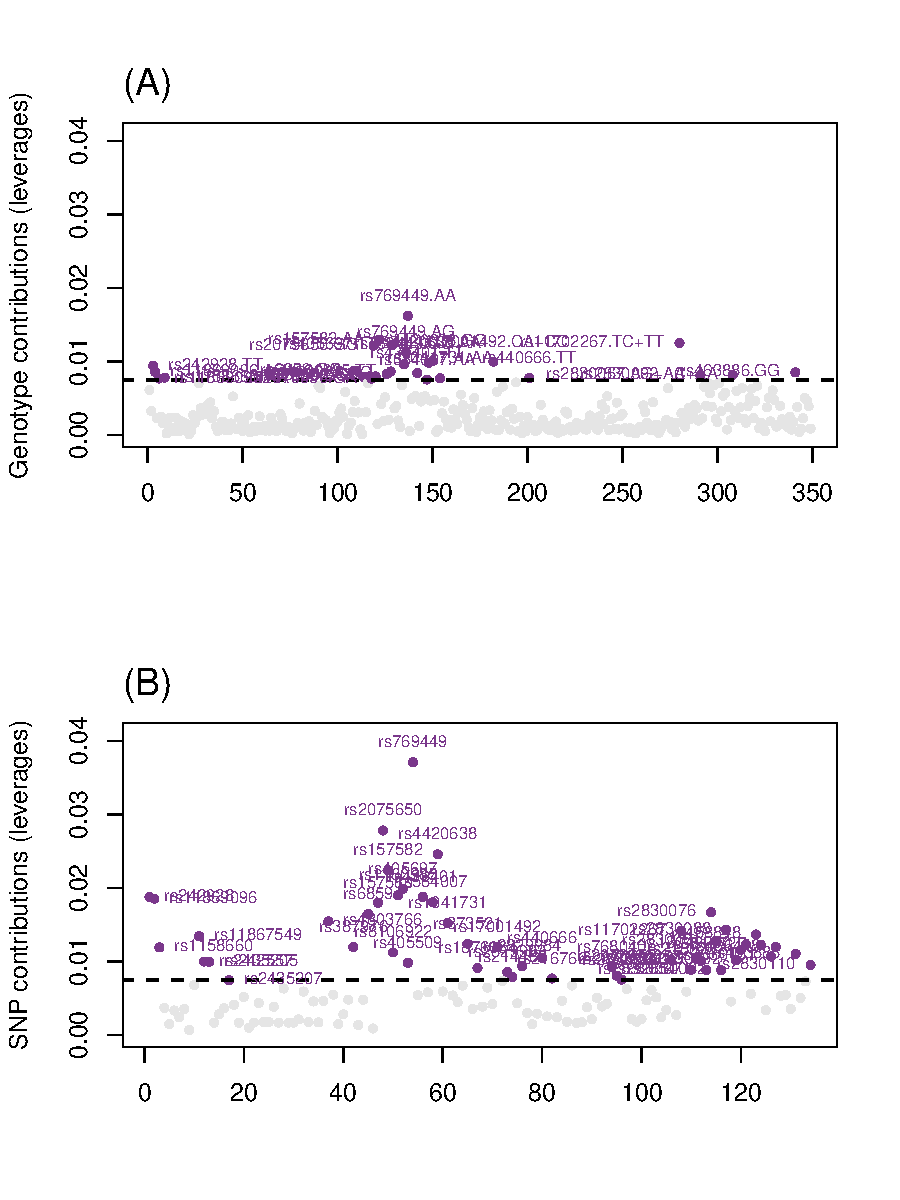
\includegraphics[width=.8\textwidth,height=.8\textheight]{PLSCAR_to_a_GPLS_files/figure-latex/unnamed-chunk-4-1} 

}

\caption{\label{fig:leverages_ex1} Regression approach to prediction of genotypes from groups. Contributions across all components for genotypes (A; top) and the SNPs (B; bottom) computed as the summation of genotypes within a SNP. The horizontal line shows the expected variance and we only highlight genotypes (A; top) or SNPs (B; bottom) greater than the expected variance. Some of the highest contributing genotypes (e.g., AA and AG genotypes for rs769449) or SNPs (e.g.,  rs769449 and rs20756560) come from the APOE and TOMM40 genes.}\label{fig:unnamed-chunk-4}
\end{figure}

Though PLS-R was initally developed as a regression
approach---especially to handle highly collinear predictors or a set of
predictors that are not full rank \citep[see explanations
in][]{wold_collinearity_1984}---it is far more common to use PLS to find
latent structures (i.e., components or latent variables)
\citep{abdi_partial_2010-1}. From this point forward we show only the
more common ``projection onto latent structures'' perspectives. We show
the latent variable scores (observations) and component scores
(variables) for the first two latent variables/components in Figure
\ref{fig:contributions_ex1}. The first latent variable scores (Fig.
\ref{fig:contributions_ex1}a) shows a gradient from the control (CN)
group through to the Alzheimer's Disease (AD) groups (CN to SMC to EMCI
to LMCI to AD). The second latent variable shows a dissociation of the
EMCI group from all other groups (Fig. \ref{fig:contributions_ex1}b).
Figure \ref{fig:contributions_ex1}c and d show the component scores for
the variables. Genotypes on the left side of first latent variable
(a.k.a., component; horizontal axis in Figs.
\ref{fig:contributions_ex1}c and d) are more associated with CN and SMC
than the other groups, where as genotypes on the right side are more
associated with AD and LMCI than the other groups. Genotypes highlighted
in purple are those that contribute more than expected variance to the
first component. Through the latent structures approach we can more
clearly see the relationships between groups and genotypes. Because we
treat the data categorically and code for genotypes, we can identify the
specific genotypes that contribute to these effects. For example the
`AA' genotype of rs769449 and the `GG' genotype of rs2075650 are more
associated with AD and LMCI than the other groups. In conrast, the `TT'
genotype of rs405697 and the `TT' genotype rs439401 are more associated
with the CN group than other groups (and thus could suggest potential
protective effects).

\begin{figure}[!hbtp]

{\centering 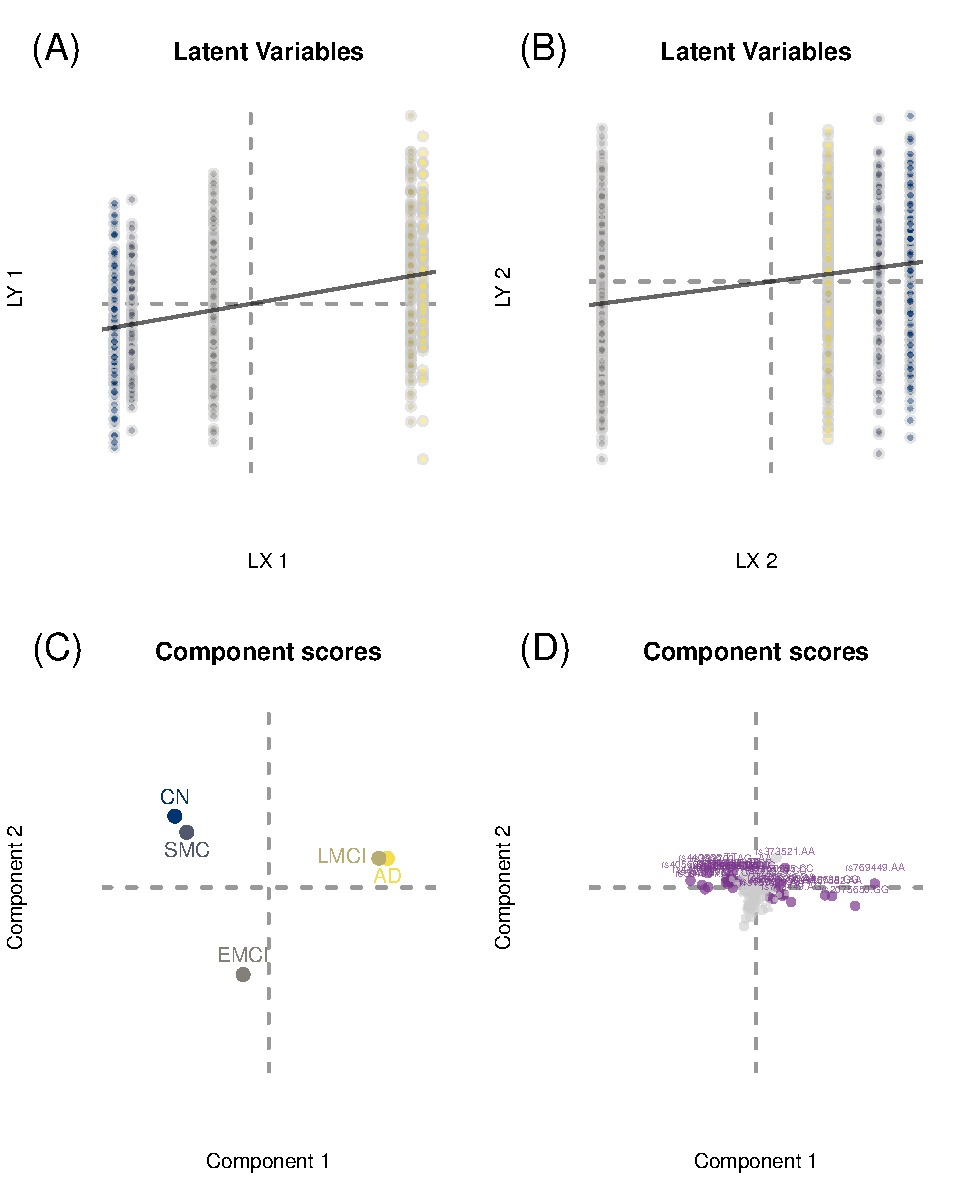
\includegraphics[width=.8\textwidth,height=.8\textheight]{PLSCAR_to_a_GPLS_files/figure-latex/unnamed-chunk-5-1} 

}

\caption{\label{fig:contributions_ex1} Latent variable projection approach to prediction of genotypes from groups. (A) and (B) show the latent variable scores for latent variables (LVs; components) one and two, respectively; (C) shows the component scores of the groups, and (D) shows the component scores of the genotypes. In (D) we highlight genotypes with above expected contribution to Latent Variable (Component) 1 in purple and make all other genotypes gray.}\label{fig:unnamed-chunk-5}
\end{figure}

\begin{figure}[!hbtp]

{\centering 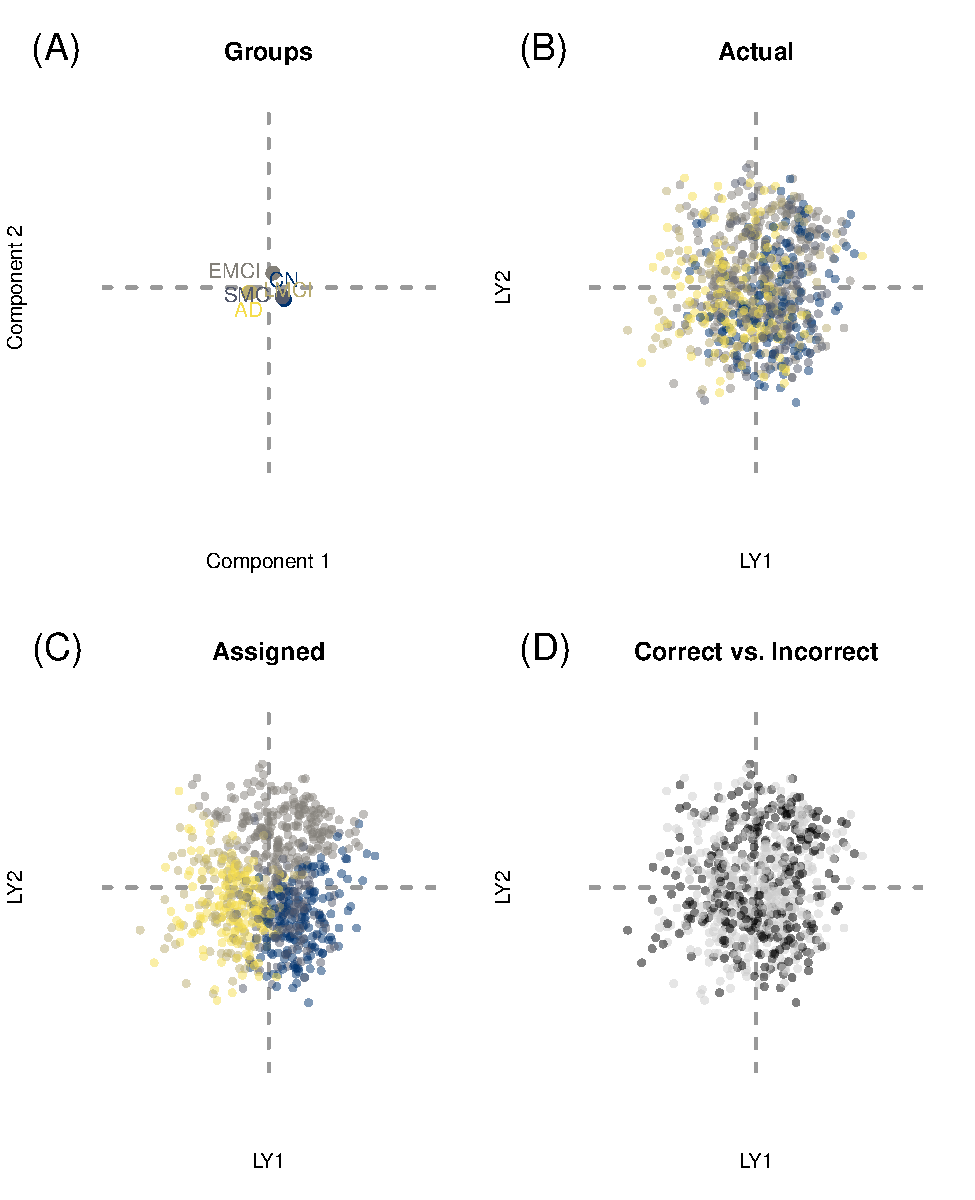
\includegraphics[width=.8\textwidth,height=.8\textheight]{PLSCAR_to_a_GPLS_files/figure-latex/unnamed-chunk-6-1} 

}

\caption{\label{fig:discriminant_ex1} Discriminant PLS-CA-R. (A) shows the component scores for the group on Latent Variables (LV) 1 and 2 (horizontal and vertical respectively), (B) shows the latent variable scores for the genotype ('LY') LV scores for LVs 1 and 2, colored by \textit{a priori} group association, (C) shows the latent variable scores for the genotype ('LY') LV scores for LVs 1 and 2, colored by \textit{assigned} group association (i.e., nearest group assignment across all LVs), and (D) shows correct vs. incorrect assignment in black and gray, respectively.}\label{fig:unnamed-chunk-6}
\end{figure}

This group-based analysis is also a discriminant analysis because it
maximally separates groups. Thus we can classify observations by
assigning them to the closest group. To correctly project observations
onto the latent variables we compute
\({\mathbf L}_{\mathbf Y} \times I^{\frac{1}{2}} = [{\bf O}_{\bf Y} \oslash ({\bf m}_{\bf Y}{\bf 1}^T)]{\bf F}_{K}\boldsymbol{\Delta}^{-1}\)
where \(1\) is a \(1 \times K\) vector of ones where
\({\bf O}_{\bf Y} \oslash ({\bf m}_{\bf Y}{\bf 1}^T)\) are ``row
profiles'' of \({\bf Y}\) (i.e., each element of \({\bf Y}\) divided by
its respective row sum). Observations from
\({\mathbf L}_{\mathbf Y} \times I^{\frac{1}{2}}\) are then assigned to
the closest group in \({\mathbf F}_{J}\), either for per component,
across a subset of components, or all components. For this example we
use the full set (four) of components. The assigned groups can then be
compared to the \emph{a priori} groups to compute a classification
accuracy. Figure \ref{fig:discriminant_ex1} shows the results of the
discriminant analysis but only visualized on the first two components.
Figures \ref{fig:discriminant_ex1}a and b show the scores for
\({\mathbf F}_{J}\) and
\({\mathbf L}_{\mathbf Y} \times I^{\frac{1}{2}}\), respectively. Figure
\ref{fig:discriminant_ex1}c shows the assignment of observations to
their closest group. Figure \ref{fig:discriminant_ex1}d visualizes the
accuracy of the assignment, where observations in black are correct
assignments (gray are incorrect assignments). The total classification
accuracy 38.69\% (where chance accuracy was 23.08\%). Finally, typical
PLS-R discriminant analyses are applied in scenarios where a small set
of, or even a single, (typically) categorical responses are predicted
from many predictors \citep{perez-enciso_prediction_2003}. However, such
an approach appears to be ``over optimistic'' in its prediction and
classification \citep{rodriguez-perez_overoptimism_2018}, which is why
we present discriminant PLS-CA-R more akin to a typical regression
problem (i.e., here a single predictor with multiple responses).

\begin{table}[!h]

\caption{\label{tab:unnamed-chunk-7}\label{table:assign_ex1} The \textit{a priori} (rows) vs. assigned (columns) accuracies for the discriminant analysis.}
\centering
\begin{tabular}[t]{lrrrrr}
\toprule
  & CN & SMC & EMCI & LMCI & AD\\
\midrule
CN & 62 & 15 & 54 & 16 & 17\\
SMC & 20 & 40 & 33 & 18 & 10\\
EMCI & 34 & 20 & 110 & 23 & 29\\
LMCI & 14 & 12 & 39 & 44 & 20\\
AD & 25 & 12 & 41 & 33 & 50\\
\bottomrule
\end{tabular}
\end{table}

\hypertarget{mixed-data-and-residualization}{%
\subsection{Mixed data and
residualization}\label{mixed-data-and-residualization}}

\label{section:mixed}

Our second example illustrates the prediction of genotypes from multiple
brain and behavioral variables: (1) three behavioral/clinical scales:
Montreal Cognitive Assessment (MoCA) \citep{nasreddine_montreal_2005},
Clinical Dementia Rating-Sum of Boxes (CDRSB)
\citep{morris1993clinical}, and Alzheimer's Disease Assessment Scale
(ADAS13) \citep{skinner_alzheimers_2012}, (2) volumetric brain measures
in \(\textrm{mm}^3\): hippocampus (HIPPO), ventricles (VENT), and whole
brain (WB), and (3) global estimates of brain function via PET scans:
average FDG (for cerebral blood flow; metabolism) in angular, temporal,
and posterior cingulate and average AV45 (A\(\beta\) tracer) standard
uptake value ratio (SUVR) in frontal, anterior cingulate, precuneus, and
parietal cortex relative to the cerebellum. This example higlights two
features of PLS-CA-R: (1) the ability to accomodate mixed data types
(continuous, ordinal, and categorical) and (2) as a way to residualize
(orthogonalize; cf.~Eq. \ref{eq:Yresid}) with respect to known or
assumed confounds.

Here, the predictors encompass a variety of data types: all of the brain
markers (volumetric MRI estimates, functional PET estimates) and the
ADAS13 appear as generally continuous data, whereas the MoCA and
especially the CDRSB are generally ordinal in part because they have
limited values constrained by a minimum and maximum score: the CDRSB
exists between 0 and 9 generally by steps of 1, and the MoCA exists
between 0 and 30, though values below 20 are exceedingly rare.
Furthermore, the assumed differences between each level are not
considered the same, for example, MoCA scores of 29 and 30 are regarded
as highly preserved and normal levels of cognition, where as 26 and 27
is the (clinical) line between impaired and unimpaired. There are many
properties of PLS-CA-R by way of CA that allow for easy inclusion of
mixed data types. In particular, continuous and ordinal data types can
be coded into what is called thermometer
\citep{beaton2018generalization}, fuzzy, or ``bipolar'' coding (because
it has two poles) \citep{greenacrefuzzy}; an idea initially propsosed by
Escofier for continuous data \citep{escofier_traitement_1979}. The
``Escofier transform'' allows continuous data to be analyzed by CA and
produces the exact same results as PCA \citep{escofier_traitement_1979}.
The same principles can be applied to ordinal data as well
\citep{beaton2018generalization}. Continuous and ordinal data can be
transformed into a ``pseudo-disjunctive'' format that behaves exactly
like complete disjunctive data (see Table \ref{table:disj}) but
preserves the values (as opposed to binning, or dichotomizing). Here, we
refer to the transform for continuous data as the ``Escofier transform''
or ``Escofier coding'' \citep{beaton_partial_2016} and the transform for
ordinal data as the ``thermometer transform'' or ``thermometer coding''.
Because continuous, ordinal, and categorical data can all be transformed
into a disjunctive-like format, they can all be analyzed with PLS-CA-R.

While the overall objective of this example is to understand the
relationship between routine markers of AD and genetics, confounds exist
for both the predictors (behavioral and brain data) and the responses
(genotype data): age, sex, and education influence the behavioral and
brain variables, whereas sex, race, and ethnicity influence the
genotypic variables. To note, these confounds are also of mixed types
(e.g., sex is categorical, age is generally continuous). Thus in this
example we illustrate the mixed analysis in two ways---unadjusted and
then adjusted for these confounds. First we show the effects of the
confounds on the separate data sets, and then compare and contrast
adjusted vs.~unadjusted analyes. For the ``mixed'' data analyses, the
volumetric data were also normalized (divided by) by intracranial volume
prior to these analyses; effectively transformed into proportional
volumes within each participant. Any other adjustments are described
when needed.

First we show the PLS-CA-R between each data set and their respective
confounds. The main effects of age, sex, and education explained 11.17\%
of the variance of the behavioral and brain data, where the main effects
of sex, race, and ethnicity explained 2.1\% of the variance of the
genotypic data. The first two components of each analysis are shown in
Figure \ref{fig:confound_predictors_ex2}. In the brain and behavioral
data, age explains a substantial amount of variance and effectively
explains Component 1. In the genotypic analysis, race is the primary
explanatory effect; more specifically, the first two components are
explained by those that identify as black or African-American (Component
1) vs.~those that identify as Asian, Native, Hawaiian, or
Latino/Hispanic (Component 2). Both data sets were reconstituted (i.e.,
\({\mathbf Y}_{\epsilon}\) from Eq. \ref{eq:Yresid}) from their
residuals.

Next we performed two analyses with the same goal: understand the
relationship between genetics and the behavioral and brain markers. In
the unadjusted analysis, the brain and behavioral data explained 1.6\%
of variance in the genotypic data, whereas in the adjusted analysis, the
brain and behavioral data explained 1.54\% of variance in the genotypic
data. The first two components of the PLS-CA-R results can be seen in
Figure \ref{fig:confound_predictors_ex2}.

\begin{figure}[!hbtp]

{\centering 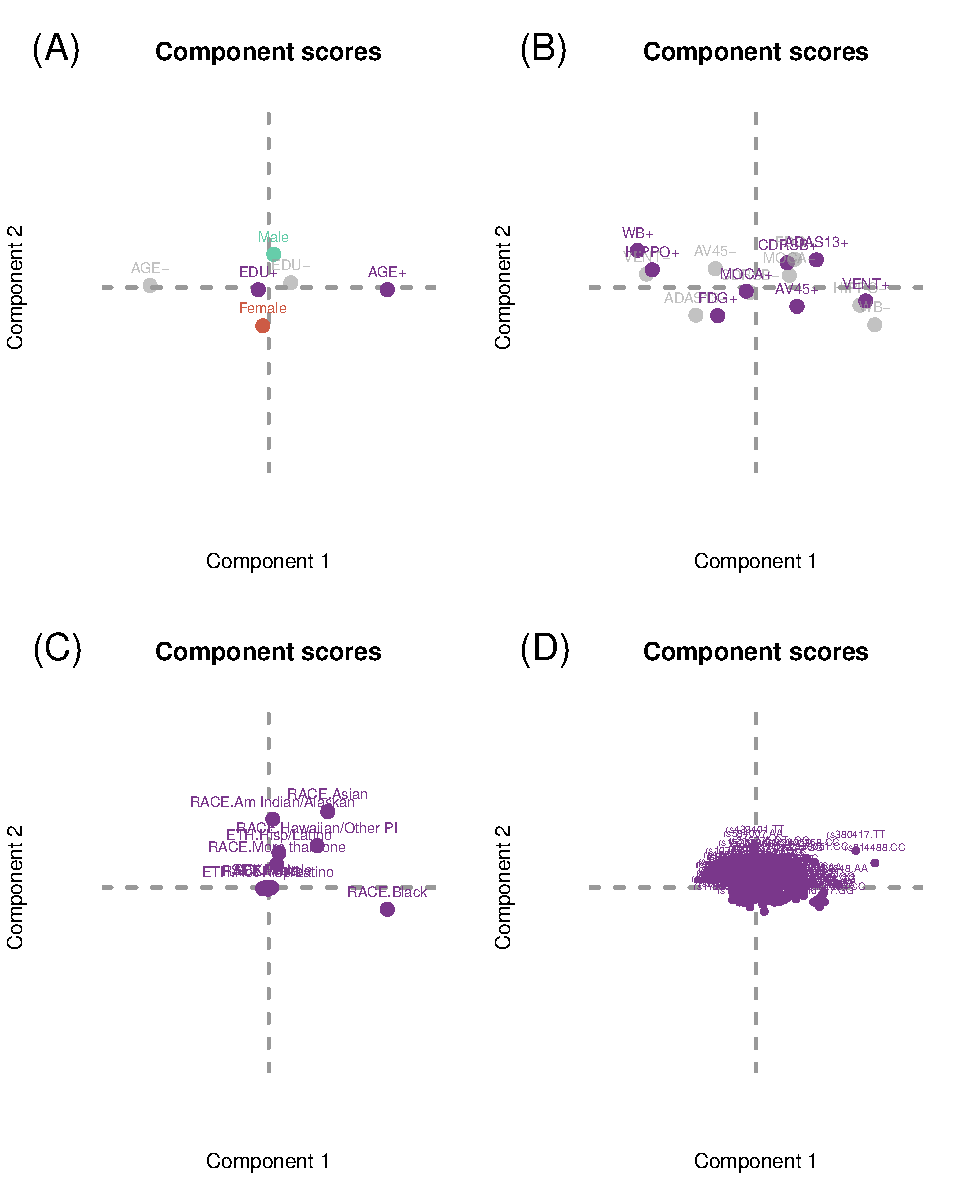
\includegraphics[width=.8\textwidth,height=.8\textheight]{PLSCAR_to_a_GPLS_files/figure-latex/unnamed-chunk-9-1} 

}

\caption{\label{fig:confound_predictors_ex2} PLS-CA-R used as a way to residualize (orthogonalize) data. The top figures (A) and (B) show prediction of the brain and behavior markers from age, sex, and education. Gray items are one side (lower end) of the "bipolar" or pseudo-disjunctive variables. The bottom figures (C) and (D) show the prediction of genotypes from sex, race, and ethnicity.}\label{fig:unnamed-chunk-9}
\end{figure}

In the unadjusted analysis (Figure \ref{fig:confound_predictors_ex2}a
and c) vs.~the adjusted analysis (Figure
\ref{fig:confound_predictors_ex2}b and d), we can some similarities and
differences, especially with respect to the behavioral and brain data.
AV45 shows little change after the residualization, and generally
explains a substantial amount of variance as it contributes highly to
the first two components in both analyses. The effects of the structural
data---especially the hippocampus---are dampened after adjustment (see
Figure \ref{fig:confound_predictors_ex2}a vs b), where the effects of
FDG and CDRSB are now (relatively) increased (see Figure
\ref{fig:confound_predictors_ex2}a vs b). On the subject level, the
differences are not substantial, but there are noticeable effects
especially with the ability to distinguish between groups (see Figure
\ref{fig:lv_compare_ex2}). One important effect is that on a spectrum
from CON to AD, we can see that the residualization has a larger impact
on the CON side, where the AD side remains somewhat homgeneous (see
Figure \ref{fig:lv_compare_ex2}c) for the brain and behavioral
variables. With respect to the genotypic LV, there is much less of an
effect (see Figure \ref{fig:lv_compare_ex2}d), wherein the observations
appear relatively unchanged. However, both pre- (horizontal axis; Figure
\ref{fig:lv_compare_ex2}d) and post- (vertical axis; Figure
\ref{fig:lv_compare_ex2}d) residualization shows that there are
individuals with unique genotypic patterns that remain unaffected by the
residualization process (i.e., those at the tails).

From this point forward we emphasize the results from the adjusted
analyses because they are more realistic in terms of how analyses are
performed. For this we refer to Figure \ref{fig:lv_compare_ex2}b---which
shows the latent variable scores for the observations and the averages
of those scores for the groups---and Figures
\ref{fig:original_residualized_ex2}b and
\ref{fig:original_residualized_ex2}d---which show the component scores
for the brain and behavioral markers and the genotypes, respectively.
The first latent variable (Fig. \ref{fig:lv_compare_ex2}b) shows a
gradient from control (CON) on the left to Alzheimer's Disease (AD) on
the right. Brain and behavioral variables on the right side of the first
component (horizontal axis in Fig. \ref{fig:original_residualized_ex2}b)
are more associated with genotypes on the right side (Fig.
\ref{fig:original_residualized_ex2}d), where brain and behavioral
variables on the left side of are more associated with genotypes on the
left side. In particular, the AA genotype of rs769449, GG genotype of
rs2075650, GG genotype of rs4420638, and AA genotype of rs157582
(amongst others) are related to increased AV45 (AV45+), decreased FDG
(FDG-), and increased ADAS13 scores (ADAS13+), where as the TT genotype
of rs405697, GG genotype of rs157580, and TC+TT genotypes of rs7412
(amongst others) are more associated with control or possibly protective
effects (i.e., decreased AV4, increased FDG, and decreased ADAS13
scores).

\begin{figure}[!hbtp]

{\centering 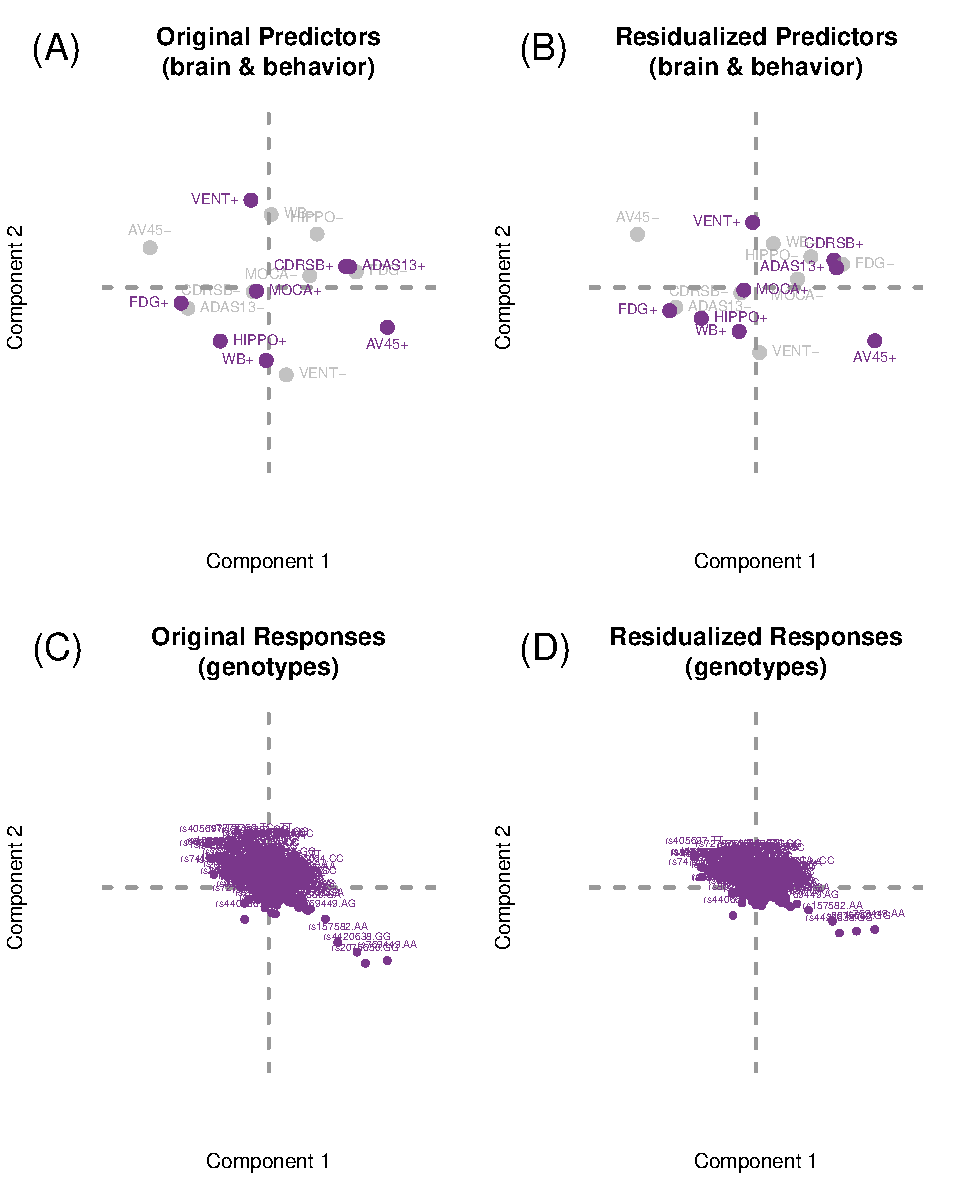
\includegraphics[width=.8\textwidth,height=.8\textheight]{PLSCAR_to_a_GPLS_files/figure-latex/unnamed-chunk-10-1} 

}

\caption{\label{fig:original_residualized_ex2} PLS-CA-R to predict genotypes from brain and behavioral markers on the original and residualized data shown on the first two latent variables (components). The top figures (A) and (B) show the component scores for the brain and behavioral markers for the original and residualized data, respectively, and the bottom figures (C) and (D) show the component scores for the genotypes for the original and residualized data, respectively.}\label{fig:unnamed-chunk-10}
\end{figure}

\begin{figure}[!hbtp]

{\centering 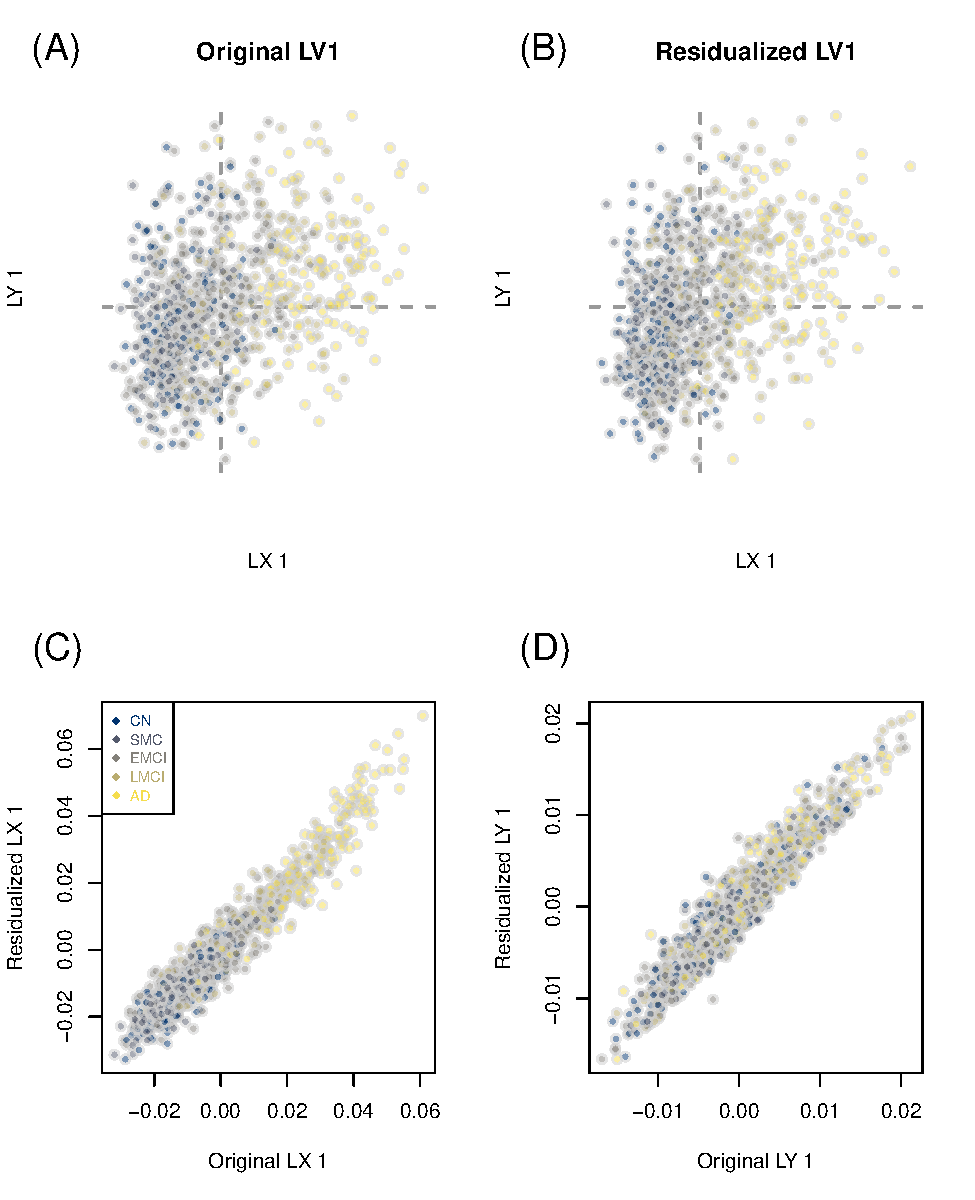
\includegraphics[width=.8\textwidth,height=.8\textheight]{PLSCAR_to_a_GPLS_files/figure-latex/unnamed-chunk-11-1} 

}

\caption{\label{fig:lv_compare_ex2} Latent variable scores (observations) for the first latent variable. The top figures (A) and (B) show the projection of the latent variable scores from each set: LX are the brain and behavioral markers, where as LY are the genotypes, for the original and residualized, respectively. The bottom figures (C) and (D) show the the original and residualized scores for the first latent variable compared to one another for each set: the brain and behavioral markers (LX) and the genotypes (LY), respectively.}\label{fig:unnamed-chunk-11}
\end{figure}

\hypertarget{suvr-and-genotypes}{%
\subsection{SUVR and genotypes}\label{suvr-and-genotypes}}

\label{section:big}

In this final example we make use of all the features of PLS-CA-R: an
example with mixed data types within and between data sets, each with
confounds (and thus require residualization). This example serves as
something more akin to the typical analysis pipeline with similar
objectives. The goal of this example is to predict genotypes from
\(\beta-\)amyloid burden (``AV45 uptake'') across regions of the cortex.
In this case, we also assume that the distribution of AV45 uptake across
cortical regions approximately follows that of \(\chi^2\) in that we
compute the deviations from independence (produced from the product
between the row and column probabilities). However we want to note that
this is only one possible way to handle such data. It is possible to
treat these data as row-wise proportions (i.e., percentage of total
uptake per region within each subject) or even as continuous data;
though these data are strictly non-negative. Ultimately, it is up to the
analyst to decide how to treat such data and how it fits into the
analysis framework.

Because not all subjects have complete AV45 and genotypic data, the
sample for this example is slightly smaller: \(N=\) 778. Ethnicity,
race, and sex (all categorical) explains 2.07\% of the variance in the
genotypic data where age (numeric), education (ordinal), and sex
(categorical) explains 2.22\% of the variance in the in the AV45 uptake
data. Overall, AV45 brain data explains 9.08\% of the variance in the
genotypic data. With the adjusted data we can now perform our intended
analyses. Although this analysis produced 67 components (latent
variables), we focus on just the first (0.57\% of genotypic variance
explained by AV45 brain data).

\begin{figure}[!hbtp]

{\centering 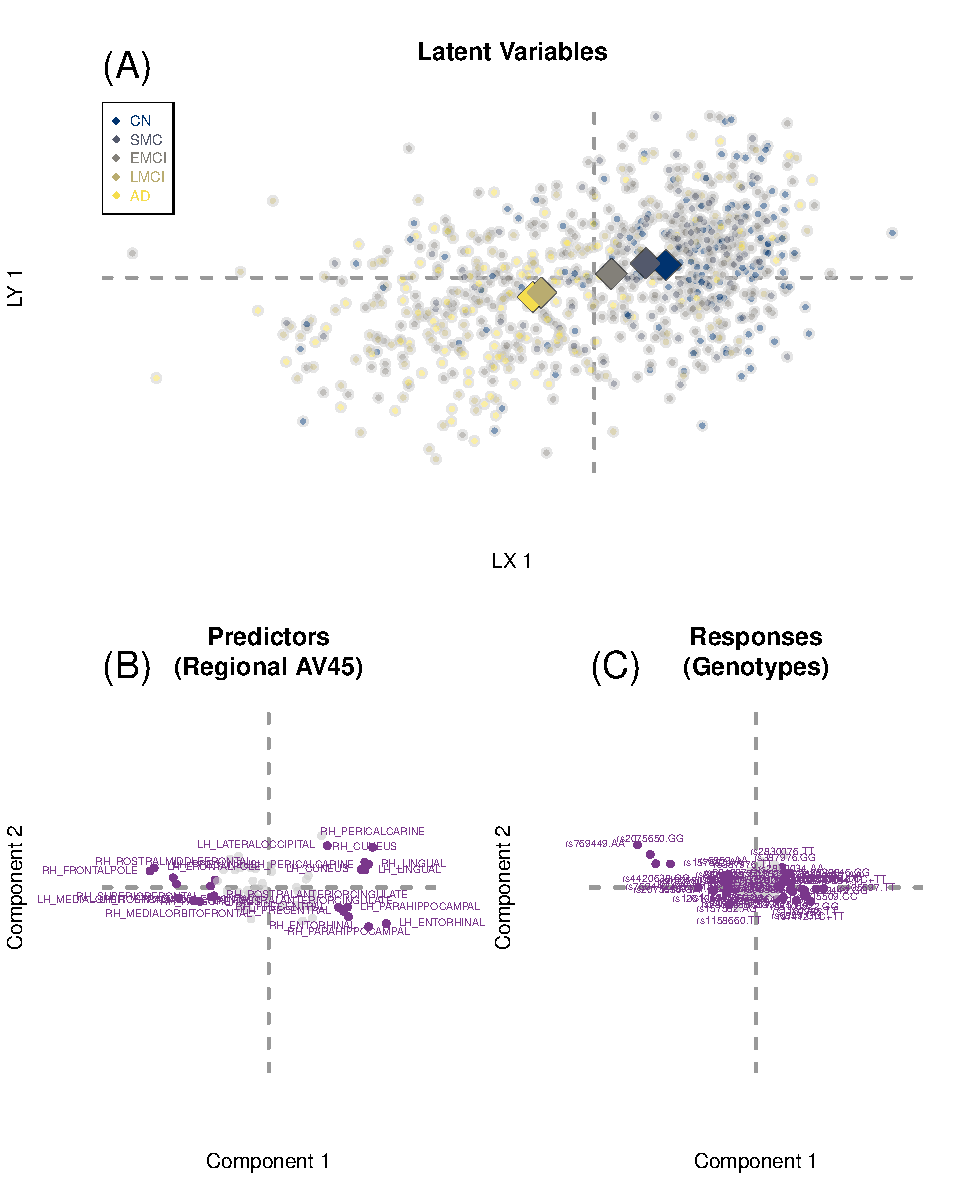
\includegraphics[width=.8\textwidth,height=.8\textheight]{PLSCAR_to_a_GPLS_files/figure-latex/unnamed-chunk-13-1} 

}

\caption{\label{fig:brain_genotypes_ex2} PLS-CA-R to predict genotypes from amyloid burden ("AV45 uptake"). The top figure (A) shows the latent variable scores for the observations on the first latent variable with group averages. The bottom figures (B) and (C) show the amyloid burden in cortical regions and the genotypes, respecively. In (A) we see a gradient from the Alzheimer's Disease (AD) group to the control (CON) group. Only items with above expected contribution to variance on the first LV are highlighed in purple.}\label{fig:unnamed-chunk-13}
\end{figure}

The first latent variable in Figure \ref{fig:brain_genotypes_ex2}a is
associated with only the horizontal axes (Component 1) in Figure
\ref{fig:brain_genotypes_ex2}b and c.~The horizontal axis in Fig.
\ref{fig:brain_genotypes_ex2}a is associated with the horizontal axis in
Fig. \ref{fig:brain_genotypes_ex2}b whereas the vertical axis in Fig.
\ref{fig:brain_genotypes_ex2}a is associated with the horizontal axis in
Fig. \ref{fig:brain_genotypes_ex2}c.~The first latent variable (Figure
\ref{fig:brain_genotypes_ex2}a) shows a gradient: from left to right we
see the groups configured from CN to AD. On the first latent variable we
do also see a group-level dissociation where AD+LMCI are entirely on one
side whereas EMCI+SMC+CN are on the opposite side for both
\({\bf L}_{\bf X}\) (AV45 uptake, horizontal) and \({\bf L}_{\bf Y}\)
(genotypes, vertical); effectively the means of AD and LMCI exist in the
upper right quadrant and the means of the EMCI, SMC, and CN groups exist
in the lower left quadrant. Higher relative AV45 uptake for the regions
on the left side of Component 1 are more associated with EMCI, SMC, and
CN than with the other groups, whereas higher relative AV45 uptake for
the regions on the right side of Component 1 are more associated with AD
and LMCI (Fig. \ref{fig:brain_genotypes_ex2}b). The genotypes on the
left side are associated with the uptake in regions on the left side and
the genotypes on the right side are associated with the uptake in
regions on the right side (Fig. \ref{fig:brain_genotypes_ex2}c). For
example, LV/Component 1 shows relative uptake in right and left frontal
pole, rostral middle frontal, and medial orbitofrontal regions are more
associated with the following genotypes: AA and AG from rs769449, GG
from rs2075650, GG from rs4420638, and AA from rs157582, than with other
genotypes; these effects are generally driven by the AD and LMCI groups.
Conversely, LV/Component 1 shows higher relative uptake in right and
left lingual, cuneus, as well left parahippocampal and left entorhinal
are more associated with the following genotypes: TT from rs405697, GG
from rs6859, TC+TT from rs7412, TT from rs2830076, GG from rs157580, and
AA from rs4420638 genotypes than with other genotypes; these effects are
generally driven by the CN, SMC, and EMCI cohorts. In summary, from the
PLS-CA-R results we see that particular patterns of regional AV45 uptake
predict particular genotypic patterns across many SNPs, and that the
sources these effects are generally driven by the groups. Furthermore
the underlying brain and genotypic effects of the groups exist along a
spectrum of severity.

\hypertarget{discussion}{%
\section{Discussion}\label{discussion}}

\label{section:Disc}

Many modern studies, like ADNI, aim to measure individuals at a variety
of scales: genetics and genomics, brain structure and function, many
aspects of cognition and behavior, batteries of clinical measures, and
almost anything in between all of these levels. These data are extremely
complex: they are heterogeneous and more often ``wide'' (many more
variables than subjects) than ``big'' (more subjects than variables).
But many current strategies and approaches to handle such multivariate
heterogeneous data often requires compromises or sacrifices (e.g., the
presumption of single numeric model for categorical data such as the
additive model for SNPs; Z-scores of ordinal values; or ``dichotomania''
(\url{https://www.fharrell.com/post/errmed/\#catg}): the binning of
continuous values into categories). Many of those strategies and
approaches presume that all data are interval scale, and therefore the
properties of those data types are effectively ignored. Because of the
many features and flexibility of PLS-CA-R---e.g., best fit to
predictors, orthogonal latent variables, accommodation for virtually any
data type---we are able to identify distinct variables and levels (e.g.,
genotypes) that define or contribute to control (CON) vs.~disease (AD)
effects (e.g., Fig. \ref{fig:contributions_ex1}) or reveal particular
patterns anchored by the polar control and disease effects (CON
\(\rightarrow\) SMC \(\rightarrow\) EMCI \(\rightarrow\) LMCI
\(\rightarrow\) AD; see, e.g., Fig. \ref{fig:brain_genotypes_ex2}).

While we focused on particular ways of coding and transforming data,
there are many alternatives that could be used with PLS-CA-R. For
example, we used a disjunctive approach for SNPs because they are
categorical, which matches the genotypic model. However, through various
disjunctive schemes, or other forms of Escofier or fuzzy coding, we
could have used any genetic model: if all SNPs were coded as the major
vs.~the minor allele (`AA' vs.~\{`Aa+aa'\}), this would be the dominant
model, or we could have assumed the additive model ---i.e., 0, 1, 2 for
`AA', `Aa', and `aa', respectively---and transformed the data with the
ordinal approach (but we strongly emphasize \emph{not} the continuous
approach). We previously provided a comprehensive guide on how to
transform various SNP genetic models for use in PLS-CA and CA elsewhere
\citep[see Appendix of][]{beaton_partial_2016}. Furthermore, we only
highlighted one of many possible methods to transform ordinal data. The
term ``fuzzy coding'' applies more generally to the recoding of ordinal,
ranked, preference, and even continuous data across a number of schemes,
all of which conform to the same properties as disjunctive data. The
many ``fuzzy'' and ``double'' coding schemes are generally found in
\citet{escofier_traitement_1979}, \citet{lebart_multivariate_1984}, or
\citet{greenacrefuzzy}. However, for ordinal data---especially with
fewer than or equal to 10 levels, and without excessively rare
(\(\leq 1\)\%) occurences---we recommend to treat ordinal values as
categorical levels. When ordinal data are treated as categorial (and
disjunctively coded), greater detail about the levels emerges and in
most cases reveal non-linear patterns of the ordinal levels.

Though we have presented PLS-CA-R as a generalization of PLS-R that
accomodates virutally any data type (by way of CA), the way we
formalized PLS-CA-R---in Section \ref{section:plscar_form} and describe
its algorithm in Algorithm \ref{algo:plscar}---leads to further variants
and broader generalizations; generalizations that span various PLS, CA,
and related approaches, several typical PLS algorithms, a variety of
optimizations (e.g., canonical correlation), and ridge-like
regularization.

\hypertarget{gpls-algorithms}{%
\subsection{GPLS algorithms}\label{gpls-algorithms}}

In general there exist three primary PLS algorithms: PLS correlation
decomposition \citep{bookstein1994partial, ketterlinus1989partial}
generally more known in neuroimaging
\citep{mcintosh_spatial_1996, mcintosh_partial_2004, krishnan_partial_2011}
which has numerous alternate names such as PLS-SVD and Tucker's
interbattery factor analysis \citep{tucker_inter-battery_1958} amongst
others \citep[see also][]{beaton_partial_2016}, PLS regression
decomposition (cf.~Section \ref{section:plscar_form} and also Algorithm
\ref{algo:plscar}) and the PLS canonical decomposition
\citep{tenenhaus_regression_1998, wegelin2000survey}, which is a
symmetric method with iterative deflation (i.e., it has features of both
PLS-C and PLS-R). Given the way in which we formalize PLS-CA-R---as a
generalized PLS-R---here we show how PLS-CA-R provides the basis of
generalizations of these three algorithms, as well as further
optimizations, similar to \citet{borga_unified_1992},
\citet{indahl2009canonical}, and \citet{de2019pls} but we do so in a
more comprehensive way that incorporates more methods than other
unification strategies, and we also do so in a way that accomodates
multiple data types. We refer to the three techniques under the umbrella
of generalized partial least squares (GPLS) as GPLS-COR, GPLS-REG, and
GPLS-CAN, for the ``correlation'', ``regression'', and ``canonical''
decompositions respectively. GPLS-COR and GPLS-CAN are symmetric
decomposition approaches where neither \({\mathbf Z}_{{\mathbf X}}\) nor
\({\mathbf Z}_{{\mathbf Y}}\) are privileged. GPLS-REG is an asymmetric
decomposition approach where \({\mathbf Z}_{{\mathbf X}}\) is
privileged. We present the GPLS-COR, GPLS-REG, and then GPLS-CAN
algorithms with their respective optimizations. We do so in the
previously mentioned order because GPLS-COR is used as the basis of all
three algorithms and GPLS-CAN shares features and concepts with both
GPLS-COR and GPLS-REG. For all of these we rely on the formlization of
PLS-CA-R we established in Section
\ref{section:plscar_form}---specifically for various mixed data types
under the \(\chi^2\) model (as used in CA).

The GPLS-COR decomposition is the simplest GPLS technique. It requires
only a single pass of the SVD---or in our case the GPLSSVD. There are no
explicit iterative steps in GPLS-COR. GPLS-COR takes as input the two
preprocessed matrices---\({\mathbf Z}_{\mathbf X}\) and
\({\mathbf Z}_{\mathbf Y}\)---and their respective row and column
weights: \({\mathbf M}_{\mathbf X}\) and \({\mathbf W}_{\mathbf X}\) for
\({\mathbf Z}_{\mathbf X}\), and \({\mathbf M}_{\mathbf Y}\) and
\({\mathbf W}_{\mathbf Y}\) for \({\mathbf Z}_{\mathbf Y}\), where \(C\)
is the desired number of components to return. GPLS-COR is shown in
Algorithm \ref{algo:plsc}.

\RestyleAlgo{boxed}
\begin{algorithm}
\DontPrintSemicolon
\SetAlgoLined
\KwResult{Generalized PLS-correlation between ${\mathbf Z}_{{\mathbf X}}$ and ${\mathbf Z}_{{\mathbf Y}}$}
\SetKwInOut{Input}{Input}\SetKwInOut{Output}{Output}
\Input{${\mathbf M}_{\mathbf{X}}$, ${\mathbf Z}_{{\mathbf X}}$, ${\mathbf W}_{\mathbf{X}}$, ${\mathbf M}_{\mathbf{Y}}$, ${\mathbf Z}_{{\mathbf Y}}$, ${\mathbf W}_{\mathbf{Y}}$, $C$}
\Output{${\mathbf U}$, ${\mathbf V}$, ${\mathbf P}$, ${\mathbf Q}$, ${\mathbf F}_{J}$, ${\mathbf F}_{K}$, ${\mathbf L}_{{\mathbf X}}$, ${\mathbf L}_{{\mathbf Y}}$, ${\boldsymbol \Delta}$}
\BlankLine
  $\mathrm{GPLSSVD(} {\mathbf M}_{\mathbf{X}}, {\mathbf Z}_{{\mathbf X}}, {\mathbf W}_{\mathbf{X}}, {\mathbf M}_{\mathbf{Y}}, {\mathbf Z}_{{\mathbf Y}}, {\mathbf W}_{\mathbf{Y}}, C \mathrm{)}$ \\
\caption{Generalized PLS-correlation algorithm. GPLS-COR is the GPLSSVD and provides the basis of other GPLS techniques. Furthermore, GPLS-COR easily allows for a variety of optmizations for examples canonical correlation, reduced rank regression (redundancy analysis), and even ridge-like regularization.}
\label{algo:plsc}
\end{algorithm}

GPLS-COR maximizes the relationship between \({\mathbf L}_{\mathbf X}\)
and \({\mathbf L}_{\mathbf Y}\) with the orthogonality constraint
\({\boldsymbol \ell}_{{\mathbf X},c}^{T}{\boldsymbol \ell}_{{\mathbf Y},c'} = 0\)
when \(c \neq c'\) where
\({\boldsymbol \ell}_{{\mathbf X},c}^{T}{\boldsymbol \ell}_{{\mathbf Y},c} = \delta_{c}\)
and thus
\({\mathbf L}_{\mathbf X}^{T}{\mathbf L}_{\mathbf Y} = {\mathbf U}^{T}\widetilde{\mathbf Z}_{\mathbf X}^{T}\widetilde{\mathbf Z}_{\mathbf Y}{\mathbf V}^{T} = {\mathbf U}^{T}\widetilde{\mathbf Z}_{\mathbf R}{\mathbf V}^{T} = {\mathbf U}^{T}{\mathbf U}{\boldsymbol \Delta}{\mathbf V}^{T}{\mathbf V}^{T} = {\boldsymbol \Delta}\).
We can show this with the generalized vectors and weight as
\({\mathbf L}_{\mathbf X}^{T}{\mathbf L}_{\mathbf Y} = {\mathbf P}^{T}{\mathbf W}_{\mathbf X}{\mathbf Z}_{\mathbf X}^{T}{\mathbf M}_{\mathbf X}^{\frac{1}{2}}{\mathbf M}_{\mathbf Y}^{\frac{1}{2}}{\mathbf Z}_{\mathbf Y}{\mathbf W}_{\mathbf Y}{\mathbf Q}^{T} = {\mathbf P}^{T}{\mathbf W}_{\mathbf X}{\mathbf P}{\boldsymbol \Delta}{\mathbf Q}^{T}{\mathbf W}_{\mathbf Y}{\mathbf Q} = {\boldsymbol \Delta}\).
Furthermore, GPLS-COR (via GPLSSVD) provides all of the other outputs as
previously described in Section \ref{section:GSVDCA}. GPLS-COR---which
is the GPLSSVD---provides the basis for the other two algorithms: both
GPLS-REG and GPLS-CAN make use of GPLS-COR (i.e., the GPLSSVD) with rank
1 solutions iteratively.

The GPLS-REG decomposition builds off of the GPLS-COR algorithm, but
does so by way of the GPLSSVD septuplet iteratively for \(C\)
iterations, with only a rank 1 solution is provided for each use of the
GPLSSVD. Then the two data matrices---\({\mathbf Z}_{\mathbf X}\) and
\({\mathbf Z}_{\mathbf Y}\)---are deflated for each step asymmetrically,
with a privileged \({\mathbf Z}_{\mathbf X}\). GPLS-REG is shown in
Algorithm \ref{algo:plscar}.

\RestyleAlgo{boxed}
\begin{algorithm}
\DontPrintSemicolon
\SetAlgoLined
\KwResult{Generalized PLS-regression between ${\mathbf Z}_{{\mathbf X}}$ and ${\mathbf Z}_{{\mathbf Y}}$}
\SetKwInOut{Input}{Input}\SetKwInOut{Output}{Output}
\Input{${\mathbf M}_{\mathbf{X}}$, ${\mathbf Z}_{{\mathbf X}}$, ${\mathbf W}_{\mathbf{X}}$, ${\mathbf M}_{\mathbf{Y}}$, ${\mathbf Z}_{{\mathbf Y}}$, ${\mathbf W}_{\mathbf{Y}}$, $C$}
\Output{$\widetilde{\mathbf U}$, $\widetilde{\mathbf V}$, $\widetilde{\mathbf P}$, $\widetilde{\mathbf Q}$, $\widetilde{\mathbf F}_{J}$, $\widetilde{\mathbf F}_{K}$, ${\mathbf L}_{{\mathbf X}}$, ${\mathbf L}_{{\mathbf Y}}$, $\widetilde{\boldsymbol \Delta}$, ${\mathbf T}_{{\mathbf X}}$, $\widehat{\mathbf U}$, ${\mathbf B}$}
\BlankLine
\For{$c=1, \dots, C$}{

  $\mathrm{GPLSSVD(} {\mathbf M}_{\mathbf{X}}, {\mathbf Z}_{{\mathbf X}}, {\mathbf W}_{\mathbf{X}}, {\mathbf M}_{\mathbf{Y}}, {\mathbf Z}_{{\mathbf Y}}, {\mathbf W}_{\mathbf{Y}}, 1 \mathrm{)}$ \\
  ${\mathbf t}_{\mathbf X} \leftarrow {\boldsymbol \ell}_{\mathbf X} \times {{\lvert\lvert {\boldsymbol \ell}_{\mathbf X} \rvert\rvert}^{-1}}$\\
  $b \leftarrow {\boldsymbol \ell}_{\mathbf Y}^{T}{\mathbf t}_{\mathbf X}$\\
  $\widehat{\mathbf u} \leftarrow ({\mathbf M}_{\mathbf X}^{\frac{1}{2}}{\mathbf Z}_{\mathbf X}{\mathbf W}_{\mathbf X}^{\frac{1}{2}})^{T}{\mathbf t}_{\mathbf X}$\\
  ${\mathbf Z}_{{\mathbf X}} \leftarrow {\mathbf Z}_{{\mathbf X}} - [{\mathbf M}_{\mathbf X}^{-\frac{1}{2}}({\mathbf t}_{\mathbf X}\widehat{\mathbf u}^{T}){\mathbf W}_{\mathbf X}^{-\frac{1}{2}}]$\\
  ${\mathbf Z}_{{\mathbf Y}} \leftarrow {\mathbf Z}_{{\mathbf Y}} - [{\mathbf M}_{\mathbf Y}^{-\frac{1}{2}}(b{\mathbf t}_{\mathbf X}\widetilde{\mathbf{v}}^{T}){\mathbf W}_{\mathbf Y}^{-\frac{1}{2}}]$
}
\caption{Generalized PLS-regression algorithm. The results of a rank 1 GPLSSVD are used to compute the latent variables and values necessary for deflation of ${\mathbf Z}_{{\mathbf X}}$ and ${\mathbf Z}_{{\mathbf Y}}$. PLS-CA-R is a specific instance of GPLS-REG, which we defined in Section \ref{section:plscar_form}.}
\label{algo:plscar}
\end{algorithm}

GPLS-REG maximizes the relationship between \({\mathbf L}_{\mathbf X}\)
and \({\mathbf L}_{\mathbf Y}\) with the orthogonality constraint
\({\boldsymbol \ell}_{{\mathbf X},c}^{T}{\boldsymbol \ell}_{{\mathbf X},c'} = 0\)
when \(c \neq c'\) where
\({\boldsymbol \ell}_{{\mathbf X},c}^{T}{\boldsymbol \ell}_{{\mathbf Y},c} = \delta_{c}\)
which is also
\(\mathrm{diag\{}{\mathbf L}_{\mathbf X}^{T}{\mathbf L}_{\mathbf Y}\mathrm{\}} = \mathrm{diag\{}\widetilde{\boldsymbol \Delta}\mathrm{\}}\).

The GPLS-CAN decomposition builds off of the GPLS-COR algorithm, but
does so by way of the GPLSSVD septuplet iteratively for \(C\)
iterations, with only a rank 1 solution is provided for each use of the
GPLSSVD. Then the two data matrices---\({\mathbf Z}_{\mathbf X}\) and
\({\mathbf Z}_{\mathbf Y}\)---are deflated for each step symmetrically.
GPLS-CAN is shown in Algorithm \ref{algo:plscacan}

\RestyleAlgo{boxed}
\begin{algorithm}
\DontPrintSemicolon
\SetAlgoLined
\KwResult{Generalized PLS-canonical between ${\mathbf Z}_{{\mathbf X}}$ and ${\mathbf Z}_{{\mathbf Y}}$}
\SetKwInOut{Input}{Input}\SetKwInOut{Output}{Output}
\Input{${\mathbf M}_{\mathbf{X}}$, ${\mathbf Z}_{{\mathbf X}}$, ${\mathbf W}_{\mathbf{X}}$, ${\mathbf M}_{\mathbf{Y}}$, ${\mathbf Z}_{{\mathbf Y}}$, ${\mathbf W}_{\mathbf{Y}}$, $C$}
\Output{$\widetilde{\mathbf U}$, $\widetilde{\mathbf V}$, $\widetilde{\mathbf P}$, $\widetilde{\mathbf Q}$, $\widetilde{\mathbf F}_{J}$, $\widetilde{\mathbf F}_{K}$, ${\mathbf L}_{{\mathbf X}}$, ${\mathbf L}_{{\mathbf Y}}$, $\widetilde{\boldsymbol \Delta}$, ${\mathbf T}_{{\mathbf X}}$, ${\mathbf T}_{{\mathbf Y}}$, $\widehat{\mathbf U}$, $\widehat{\mathbf V}$}
\BlankLine
\For{$c=1, \dots, C$}{

  $\mathrm{GPLSSVD(} {\mathbf M}_{\mathbf{X}}, {\mathbf Z}_{{\mathbf X}}, {\mathbf W}_{\mathbf{X}}, {\mathbf M}_{\mathbf{Y}}, {\mathbf Z}_{{\mathbf Y}}, {\mathbf W}_{\mathbf{Y}}, 1 \mathrm{)}$ \\
  ${\mathbf t}_{\mathbf X} \leftarrow {\boldsymbol \ell}_{\mathbf X} \times {{\lvert\lvert {\boldsymbol \ell}_{\mathbf X} \rvert\rvert}^{-1}}$\\
  ${\mathbf t}_{\mathbf Y} \leftarrow {\boldsymbol \ell}_{\mathbf Y} \times {{\lvert\lvert {\boldsymbol \ell}_{\mathbf Y} \rvert\rvert}^{-1}}$\\
  $\widehat{\mathbf u} \leftarrow ({\mathbf M}_{\mathbf X}^{\frac{1}{2}}{\mathbf Z}_{\mathbf X}{\mathbf W}_{\mathbf X}^{\frac{1}{2}})^{T}{\mathbf t}_{\mathbf X}$\\
  $\widehat{\mathbf v} \leftarrow ({\mathbf M}_{\mathbf Y}^{\frac{1}{2}}{\mathbf Z}_{\mathbf Y}{\mathbf W}_{\mathbf Y}^{\frac{1}{2}})^{T}{\mathbf t}_{\mathbf Y}$\\  
  
  ${\mathbf Z}_{{\mathbf X}} \leftarrow {\mathbf Z}_{{\mathbf X}} - [{\mathbf M}_{\mathbf X}^{-\frac{1}{2}}({\mathbf t}_{\mathbf X}\widehat{\mathbf u}^{T}){\mathbf W}_{\mathbf X}^{-\frac{1}{2}}]$\\
   ${\mathbf Z}_{{\mathbf Y}} \leftarrow {\mathbf Z}_{{\mathbf Y}} - [{\mathbf M}_{\mathbf Y}^{-\frac{1}{2}}({\mathbf t}_{\mathbf Y}\widehat{\mathbf v}^{T}){\mathbf W}_{\mathbf Y}^{-\frac{1}{2}}]$
}
\caption{Generalized PLS-canonical algorithm. The results of a rank 1 GPLSSVD are used to compute the latent variables and values necessary for deflation of ${\mathbf Z}_{{\mathbf X}}$ and ${\mathbf Z}_{{\mathbf Y}}$. Note that the deflation in GPLS-CAN differs from GPLS-REG in Algorithm \ref{algo:plscar}.}
\label{algo:plscacan}
\end{algorithm}

GPLS-CAN maximizes the relationship between \({\mathbf L}_{\mathbf X}\)
and \({\mathbf L}_{\mathbf Y}\) with the orthogonality constraints
\({\boldsymbol \ell}_{{\mathbf X},c}^{T}{\boldsymbol \ell}_{{\mathbf X},c'} = 0\)
and
\({\boldsymbol \ell}_{{\mathbf Y},c}^{T}{\boldsymbol \ell}_{{\mathbf Y},c'} = 0\)
when \(c \neq c'\) where
\({\boldsymbol \ell}_{{\mathbf X},c}^{T}{\boldsymbol \ell}_{{\mathbf Y},c} = \delta_{c}\)
which is also
\(\mathrm{diag\{}{\mathbf L}_{\mathbf X}^{T}{\mathbf L}_{\mathbf Y}\mathrm{\}} = \mathrm{diag\{}\widetilde{\boldsymbol \Delta}\mathrm{\}}\).

Note that across all three algorithms defined here, that the first
component is identical when the same preprocessed data and constraints
are provided to the GPLSSVD. In nearly all cases, subsequent components
across the three algorithms differ, but also generally they do not
differ substantially. The similarities can be traced back to the common
maximization of
\({\boldsymbol \ell}_{{\mathbf X},c}^{T}{\boldsymbol \ell}_{{\mathbf Y},c} = \delta_{c}\),
where the differences can be traced back to the specific orthogonality
optimizations when \(c \neq c'\) where: (1) GPLS-COR in Algorithm
\ref{algo:plsc} is
\({\boldsymbol \ell}_{{\mathbf X},c}^{T}{\boldsymbol \ell}_{{\mathbf Y},c'} = 0\),
(2) GPLS-REG in Algorithm \ref{algo:plscar} is
\({\boldsymbol \ell}_{{\mathbf X},c}^{T}{\boldsymbol \ell}_{{\mathbf X},c'} = 0\),
and (3) GPLS-CAN in Algorithm \ref{algo:plscacan} is both
\({\boldsymbol \ell}_{{\mathbf X},c}^{T}{\boldsymbol \ell}_{{\mathbf X},c'} = 0\)
and
\({\boldsymbol \ell}_{{\mathbf Y},c}^{T}{\boldsymbol \ell}_{{\mathbf Y},c'} = 0\).

\hypertarget{gpls-optimizations-and-further-generalizations}{%
\subsection{GPLS optimizations and further
generalizations}\label{gpls-optimizations-and-further-generalizations}}

From the GPLS perspective, we can better unify the wide variety of
approaches with similar goals but variations of metrics,
transformations, and optimizations that often appear under a wide
variety of names (e.g., PLS, CCA, interbattery factor analysis,
co-inertia analysis, canonical variates, PLS-CA, and so on; see
\citet{abdi2017canonical}). The way we defined the GPLS algorithms---in
particular with the constraints applied to the rows and columns of each
data matrix---leads to numerous further generalizations.

For simplicity, let us first focus on Algorithm \ref{algo:plsc}, and
assume that \({\mathbf X}\) and \({\mathbf Y}\) are continuous data,
where \({\mathbf Z}_{\mathbf X}\) and \({\mathbf Z}_{\mathbf Y}\) are
column-wise centered and/or scaled versions of \({\mathbf X}\) and
\({\mathbf Y}\). Though we have established Algorithm \ref{algo:plsc} as
GPLS-COR---and more generally as the GPLSSVD---we can obtain the results
of three of the most common ``two-table'' techniques: PLS correlation
(PLSC), canonical correlation analysis (CCA), and redundancy analysis
(RDA, a.k.a., reduced rank regression {[}RRR{]}). Standard PLSC is
performed as
\(\mathrm{GPLSSVD(} {\mathbf I}, {\mathbf Z}_{{\mathbf X}}, {\mathbf I}, {\mathbf I}, {\mathbf Z}_{{\mathbf Y}}, {\mathbf I}\mathrm{)}\),
CCA is performed as
\(\mathrm{GPLSSVD(} {\mathbf I}, {\mathbf Z}_{{\mathbf X}}, ({\mathbf Z}_{\mathbf X}^{T}{\mathbf Z}_{\mathbf X})^{-1}, {\mathbf I}, {\mathbf Z}_{{\mathbf Y}}, ({\mathbf Z}_{\mathbf Y}^{T}{\mathbf Z}_{\mathbf Y})^{-1}\mathrm{)}\),
and RDA---where \({\mathbf X}\) is privileged---is performed as
\(\mathrm{GPLSSVD(} {\mathbf I}, {\mathbf Z}_{{\mathbf X}}, ({\mathbf Z}_{\mathbf X}^{T}{\mathbf Z}_{\mathbf X})^{-1}, {\mathbf I}, {\mathbf Z}_{{\mathbf Y}}, {\mathbf I}\mathrm{)}\).
Furthermore, these three variants---PLSC, CCA, and RDA/RRR---also
generalize discriminant analyses under different optimizations so long
as \({\mathbf X}\) is a dummy-coded or complete disjunctive matrix to
assign each observation (row) to a specific group or category (columns).

Most importantly, because of the ways we formalized the GPLS
algorithms---see also Section \ref{section:plscar_form}---and the
variety of ways to suitably transform data (e.g., the various coding
schemes we have shown) allow application of PLS-CA-R and GPLS algorithms
on a variety of different problems or models such as log or power
transformations and alternate choices for weights (see Eq.
\ref{eq:weightmats_v1}) or models (see Eq. \ref{eq:models}). That means
that the GPLS algorithms further generalize many approaches, especially
the numerous variants of CA. Generally in the cases of strictly positive
data, there may be a need to preprocess data within the family of power
transformations for CA \citep{greenacre2009power} or alternate distance
metrics such as Hellinger distance
\citep{rao1995review, escofier1978analyse}. Finally, with the choices of
weights can change, as they do for Hellinger CA, and for the variations
of ``non-symmetrical CA''
\citep{d1992non, kroonenberg1999nonsymmetric, takane1991relationships},
where both types of variants require one set of weights as
\({\mathbf I}\) (akin to RDA/RRR-type optimizations with CA/\(\chi^2\)
models across any of the GPLS algorithms).

\hypertarget{ridge-like-regularization}{%
\subsection{Ridge-like regularization}\label{ridge-like-regularization}}

It is also possible to apply ridge-like regularization to PLS-CA
regression, correlation, and canonical decompositions. We show two
possible strategies for ridge-like regularization under the data/model
assumptions and the preprocessing we established in Section
\ref{section:plscar_form}.

The first approach is based on Takane's regularized multiple CA
\citep{takane_regularized_2006} and regularized nonsymmetric CA
\citep{takane_regularized_2009-1}. To do so, it is convenient to
slightly reformulate PLS-CA-R, but we still require \({\mathbf X}\),
\({\mathbf Y}\), \({\mathbf O}_{\mathbf X}\),
\({\mathbf O}_{\mathbf Y}\), \({\mathbf E}_{\mathbf X}\), and
\({\mathbf E}_{\mathbf Y}\) as defined in Section
\ref{section:plscar_form}. First we re-define
\({\mathbf Z}_{\mathbf X} = ({\mathbf O}_{\mathbf X} - {\mathbf E}_{\mathbf X}) \times (\mathbf{1}^{T}{\mathbf X1})\)
and
\({\mathbf Z}_{\mathbf Y} = ({\mathbf O}_{\mathbf Y} - {\mathbf E}_{\mathbf Y}) \times (\mathbf{1}^{T}{\mathbf Y1})\);
which are the same as in Eq. \ref{eq:plscar_Zs} except scaled by the
grand sum of its respective source data matrix. Next we define the
following additional matrices:
\({\mathbf D}_{{\mathbf X},I} = \mathrm{diag\{ \mathbf{X1} \}}\), and
\({\mathbf D}_{{\mathbf Y},I} = \mathrm{diag\{ \mathbf{Y1} \}}\) which
are diagonal matrices of the row sums of \({\mathbf X}\) and
\({\mathbf Y}\), respectively and
\({\mathbf D}_{{\mathbf X},J} = \mathrm{diag\{ \mathbf{1}^{T} \mathbf{X} \}}\),
and
\({\mathbf D}_{{\mathbf Y},K} = \mathrm{diag\{ \mathbf{1}^{T}\mathbf{Y} \}}\)
which are the column sums of \({\mathbf X}\) and \({\mathbf Y}\). Then
PLS-CA correlation, regression, and canonical decompositions replace the
GPLSSVD step in Algorithms \ref{algo:plsc}, \ref{algo:plscar},
\ref{algo:plscacan} with
\(\mathrm{GPLSSVD(}{\mathbf D}_{{\mathbf X},I}^{-1},{\mathbf Z}_{\mathbf X}^{T}, {\mathbf D}_{{\mathbf X},J}^{-1}, {\mathbf D}_{{\mathbf Y},I}^{-1},{\mathbf Z}_{\mathbf Y}^{T}, {\mathbf D}_{{\mathbf Y},K}^{-1} \mathrm{)}\).
The only differences between this Takane-ian reformulation and what we
originally established is that the generalized singular vectors
(\({\mathbf P}\) and \({\mathbf Q}\)) and the component scores
(\({\mathbf F}_{\mathbf J}\) and \({\mathbf F}_{\mathbf K}\)) differ by
constant scaling factors (which are the sums of \({\mathbf X}\) and
\({\mathbf Y}\) for their respective scores).

We can regularize PLS-CA-R in the same way as Takane's RMCA. We require
(1) a ridge parameter which we refer to as \(\lambda\) and (2) variants
of \({\mathbf D}_{{\mathbf X},I}\), \({\mathbf D}_{{\mathbf X},J}\),
\({\mathbf D}_{{\mathbf Y},I}\), and \({\mathbf D}_{{\mathbf Y},K}\)
that we refer to as
\({\mathbb D}_{{\mathbf X},I} = {\mathbf D}_{{\mathbf X},I} + [\lambda \times ({\mathbf Z}_{\mathbf X}{\mathbf Z}_{\mathbf X}^{T})^{+}]\),
\({\mathbb D}_{{\mathbf Y},I} = {\mathbf D}_{{\mathbf Y},I} + [\lambda \times ({\mathbf Z}_{\mathbf Y}{\mathbf Z}_{\mathbf Y}^{T})^{+}]\),
\({\mathbb D}_{{\mathbf X},J} = {\mathbf D}_{{\mathbf X},J} + [\lambda \times {\mathbf Z}_{\mathbf X}^{T}({\mathbf Z}_{\mathbf X}{\mathbf Z}_{\mathbf X}^{T})^{+}{\mathbf Z}_{\mathbf X}]\),
and
\({\mathbb D}_{{\mathbf Y},K} = {\mathbf D}_{{\mathbf Y},K} + [\lambda \times {\mathbf Z}_{\mathbf Y}^{T}({\mathbf Z}_{\mathbf Y}{\mathbf Z}_{\mathbf Y}^{T})^{+}{\mathbf Z}_{\mathbf Y}]\).
When \(\lambda = 0\) then
\({\mathbb D}_{{\mathbf X},I} = {\mathbf D}_{{\mathbf X},I}\),
\({\mathbb D}_{{\mathbf Y},I} = {\mathbf D}_{{\mathbf Y},I}\),
\({\mathbb D}_{{\mathbf X},J} = {\mathbf D}_{{\mathbf X},J}\),
\({\mathbb D}_{{\mathbf Y},K} = {\mathbf D}_{{\mathbf Y},K}\). We obtain
regularized forms of PLS-CA for the correlation, regression, and
canonical decompositions if we simply replace the GPLSSVD step in each
algorithm with
\(\mathrm{GPLSSVD(}{\mathbb D}_{{\mathbf X},I}^{-1},{\mathbf Z}_{\mathbf X}^{T}, {\mathbb D}_{{\mathbf X},J}^{-1}, {\mathbb D}_{{\mathbf Y},I}^{-1},{\mathbf Z}_{\mathbf Y}^{T}, {\mathbb D}_{{\mathbf Y},K}^{-1} \mathrm{)}\).
As per Takane's recommendation \citep{takane_regularized_2006},
\(\lambda\) could be any positive value, though integers in the range
from 1 to 20 provide sufficient regularization, especially as
\(\lambda\) increases.

But the Takane-ian approach may not be feasible when \(I\), \(J\),
and/or \(K\) are particularly large because the various crossproduct and
projection matrices require a large amount of memory and/or
computational expense. So we now introduce a ``truncated'' version of
the Takane regularization which is more computationally efficient, and
analogous to the regularization procedure of Allen
\citep{allen_sparse_2013, allen_generalized_2014}. We re-define
\({\mathbb D}_{{\mathbf X},I} = {\mathbf D}_{{\mathbf X},I} + (\lambda \times {\mathbf I})\)
and
\({\mathbb D}_{{\mathbf Y},I} = {\mathbf D}_{{\mathbf Y},I} + (\lambda \times {\mathbf I})\)
and then also
\({\mathbb D}_{{\mathbf X},J} = {\mathbf D}_{{\mathbf X},J} + (\lambda \times {\mathbf I})\)
and
\({\mathbb D}_{{\mathbf Y},K} = {\mathbf D}_{{\mathbf Y},K} + (\lambda \times {\mathbf I})\)
where \({\mathbf I}\) are identity matrices (\(1\)s on the diagonal) of
appropriate size. Like in the previous formulation, we replace the
values we have in the GPLSSVD step where
\(\mathrm{GPLSSVD(}{\mathbb D}_{{\mathbf X},I}^{-1},{\mathbf Z}_{\mathbf X}^{T}, {\mathbb D}_{{\mathbf X},J}^{-1}, {\mathbb D}_{{\mathbf Y},I}^{-1},{\mathbf Z}_{\mathbf Y}^{T}, {\mathbb D}_{{\mathbf Y},K}^{-1} \mathrm{)}\);
and in this particular case, the constraint matrices are all diagonal
matrices, which allows for a lower memory footprint and less
computational burden.

Finally, we have two concluding remarks on ridge-like regularization.
The first point is that the more simplified Takane/Allen hybrid approach
to ridge-like regularization also applies much more generally to
virtually any technique for the SVD or GPLSSVD. For any approach, we
only require some inflation factor (\(\lambda\)) for the constraints
alon the diagonals. The second point is that while we have presented
ridge-like regularization with a single \(\lambda\) it is entirely
possible to use different \(\lambda\)s for each set of constraints. But
even though it is possible, we do not recommend this approach, as it
would require a complex grid search over all the various \(\lambda\)
parameters. Alternatively, if multiple \(\lambda\)s were used, one could
minimize the number of parameters to search and set some of the
\(\lambda\)s to 0 and, for example, use only one or two \(\lambda\)
values instead of four possible \(\lambda\) values.

\hypertarget{conclusions}{%
\subsection{Conclusions}\label{conclusions}}

The primary motivation to develop PLS-CA-R was to address the need of
many fields that require \textit{data type general} methods. We
introduced PLS-CA-R in a way that emphasizes various recoding schemes to
accomodate different data types all with respect to CA and the
\(\chi^2\) model. While that was the bulk of this work, our secondary
goal was to further generalize the PLS-CA approach and to better unify
many methods under a simpler framework, specifically by way of the
GPLSSVD and our three GPLS algorithms. Thus our generalizations---first
established in Section \ref{section:plscar_form}, and expanded upon in
Discussion---accomodate: almost any data type, various metrics (e.g.,
Hellinger distance), various optimizations (e.g., PLS, CCA, or RDA type
optmizations), and even two strategies for ridge-like regularization. We
have foregone any discussions of inference, stability, and resampling
for PLS-CA-R because, as a generalization of PLS-R, many inference and
stability approaches still apply---such as feature selection or
sparsification \citep{sutton_sparse_2018}, additional regularization or
sparsification approaches
\citep{le_floch_significant_2012-1, guillemot2019constrained, tenenhaus_variable_2014, tenenhaus_regularized_2011},
cross-validation
\citep{wold_principal_1987, rodriguez-perez_overoptimism_2018, kvalheim_number_2019, abdi_partial_2010-1},
permutation \citep{berry_permutation_2011}, various bootstrap
\citep{efron_bootstrap_1979, chernick_bootstrap_2008} approaches
\citep{abdi_partial_2010-1, takane_regularized_2009-1} or tests
\citep{mcintosh_partial_2004, krishnan_partial_2011}, and other
frameworks such as split-half resampling
\citep{strother_quantitative_2002-1, kovacevic2013revisiting, strother2004optimizing}---and
are easily adapted for the PLS-CA-R and GPLS frameworks.

PLS-CA-R was designed primarily as the mixed-data generalization of PLSR
that provides for us a technique that both produces latent variables and
performs regression when standard assumptions are not met (e.g., HDLSS
or high collinearity). PLS-CA-R---and GPLS---addresses the need of many
fields that require \textit{data type general} methods across
multi-source and multi-domain data sets where we require careful
considerations about how we prepare and understand our data
\citep{nguyen2019ten}. We introduced PLS-CA-R in a way that emphasizes
various recoding schemes to accomodate different data types all with
respect to CA and the \(\chi^2\) model. PLS-CA-R provides key features
necessary for data analyses as data-rich and data-heavy disciplines and
fields rapidly move towards and depend on fundamental techniques in
machine and statistical learning (e.g., PLSR, CCA). Finally, with
techniques such as mixed-data MFA \citep{becue-bertaut_multiple_2008},
PLS-CA-R provides a much needed basis for development of future methods
designed forsuch complex data sets.

\hypertarget{acknowledgements}{%
\section{Acknowledgements}\label{acknowledgements}}

Data collection and sharing for this project was funded by the
Alzheimer's Disease Neuroimaging Initiative (ADNI) (National Institutes
of Health Grant U01 AG024904) and DOD ADNI (Department of Defense award
number W81XWH-12-2-0012). ADNI is funded by the National Institute on
Aging, the National Institute of Biomedical Imaging and Bioengineering,
and through generous contributions from the following: AbbVie,
Alzheimer's Association; Alzheimer's Drug Discovery Foundation; Araclon
Biotech; BioClinica, Inc.; Biogen; Bristol-Myers Squibb Company;
CereSpir, Inc.; Cogstate; Eisai Inc.; Elan Pharmaceuticals, Inc.; Eli
Lilly and Company; EuroImmun; F. Hoffmann-La Roche Ltd and its
affiliated company Genentech, Inc.; Fujirebio; GE Healthcare; IXICO
Ltd.; Janssen Alzheimer Immunotherapy Research \& Development, LLC.;
Johnson \& Johnson Pharmaceutical Research \& Development LLC.;
Lumosity; Lundbeck; Merck \& Co., Inc.; Meso Scale Diagnostics, LLC.;
NeuroRx Research; Neurotrack Technologies; Novartis Pharmaceuticals
Corporation; Pfizer Inc.; Piramal Imaging; Servier; Takeda
Pharmaceutical Company; and Transition Therapeutics. The Canadian
Institutes of Health Research is providing funds to support ADNI
clinical sites in Canada. Private sector contributions are facilitated
by the Foundation for the National Institutes of Health (www.fnih.org).
The grantee organization is the Northern California Institute for
Research and Education, and the study is coordinated by the Alzheimer's
Therapeutic Research Institute at the University of Southern California.
ADNI data are disseminated by the Laboratory for Neuro Imaging at the
University of Southern California.

\bibliographystyle{agsm}
\bibliography{plscar.bib}

\end{document}
